% -*- TeX:UTF-8 -*-
%%
%% KAIST 학위논문양식 LaTeX용 (ver 0.4) 예시
%%
%% @version 0.4
%% @author  채승병 Chae,Seungbyung (mailto:chess@kaist.ac.kr)
%% @date    2004. 11. 12.
%%
%% @requirement
%% teTeX, fpTeX, teTeX 등의 LaTeX2e 배포판
%% + 은광희 님의 HLaTeX 0.991 이상 버젼 또는 홍석호 님의 HPACK 1.0
%% : 설치에 대한 자세한 정보는 http://www.ktug.or.kr을 참조바랍니다.
%%
%% @note
%% 기존에 널리 쓰여오던 차재춘 님의 학위논문양식 클래스 파일의 형식을
%% 따르지 않고 전면적으로 다시 작성하였습니다. 논문 정보 입력부분에서
%% 과거 양식과 다른 부분이 많으니 아래 예시에 맞춰 바꿔주십시오.
%% 버그 리포트는 http://gsa.kaist.ac.kr/thesis-form으로 보내주십시오.
%%
%% @acknowledgement
%% 본 예시 논문은 물리학과 박사과정 김용현 님의 호의로 제공되었습니다.
%%
%% -------------------------------------------------------------------
%% @information
%% 이 예제 파일은 hangul-ucs를 사용합니다. UTF-8 입력 인코딩으로
%% 작성되었습니다. hlatex의 hfont는 이용하지 않습니다. --2006/02/11

% @class kaist.cls
% @options [default: doctor, korean, final]
% - doctor: 박사과정 | master : 석사과정
% - korean: 한글논문 | english: 영문논문
% - final : 최종판   | draft  : 시험판
% - pdfdoc : 선택하지 않으면 북마크와 colorlink를 만들지 않습니다.
\documentclass[master,english,final]{kaist-ucs}

% kaist.cls 에서는 기본으로 dhucs, ifpdf, graphicx 패키지가 로드됩니다.
% 추가로 필요한 패키지가 있다면 주석을 풀고 적어넣으십시오,
%\usepackage{...}
\usepackage{color}
\usepackage{amsmath}
\usepackage{graphicx}
\usepackage{pdflscape}
\usepackage{hyperref}
\usepackage{multirow}
\usepackage{subfig}

% @command title 논문 제목
% @options [default: (none)]
% - korean: 한글제목 | english: 영문제목
\title[korean] {이족 보행 동역학의\linebreak 생체 역학적인 접근방법}
%\title[english]{Spectral-based Shape Correspondence \linebreak with Diffusion Geometry}
\title[english]{A Biomechanical Approach to Biped Dynamics}

% @note 표지에 출력되는 제목을 강제로 줄바꿈하려면 \linebreak 을 삽입.
%       \\ 나 \newline 등을 사용하면 안됩니다. (아래는 예시)
%\title[korean]{탄소 나노튜브의 물리적 특성에 대한\linebreak 이론 연구}
%\title[english]{Theoretical study on physical properties of\linebreak
%                carbon nanotubes}

% @command author 저자 이름
% @param   family_name, given_name 성, 이름을 구분해서 입력
% @options [default: (none)]
% - korean: 한글이름 | chinese: 한문이름 | english: 영문이름
\author[korean] {김}{거 엽}
\author[chinese]{金}{거 엽}
\author[english]{Kim}{Geo Yeob}

% @command advisor 지도교수 이름 (복수가능)
% @usage   \advisor[options]{...한글이름...}{...영문이름...}{signed|nosign}
% @options [default: major]
% - major: 주 지도교수  | coopr: 공동 지도교수
\advisor[major]{신 성 용}{Shin, Sung Yong}{signed}
%\advisor[coopr]{홍 길 동}{Gil-Dong Hong}{nosign}

% @command department 학과이름 - 아래 표에 따라 코드를 입력
%
% 물리 PH
% 수리과학 MAS
% 화학 CH
% 생명과학 BS
% 바이오및뇌공학 BiS
% 의과학대학원 MSE
% 의과학학제 BM
% 기계공학 ME
% 항공우주공학 AE
% 건설 및 환경공학 CE
% 산업디자인 ID
% 생명화학공학 CBE
% 신소재공학 MS
% 원자력 및 양자 NQE
% 자동차기술대학원 AT
% 전기및전자공학 EE
% 전산학 CS
% 산업 및 시스템공학 IE
% 반도체학제 STE
% 소프트웨어 프로그램 SEP
% 정보통신학제 TE
% 고분자학학제 PSE
% 과학기술학학제 STS
% 나노과학기술학제 NT
% 로봇공학학제 RE
% 문화기술학제 CT
% 환경·에너지공학학제 ENV
% e-매뉴팩쳐링리더십학제 EML
% 문화기술대학원 GCT
% 경영공학 MT
% 테크노경영 TM
% 금융 FIN

\department{CS}

% @command studentid 학번
\studentid{20084004}

% @command referee 심사위원 (석사과정 3인, 박사과정 5인)
\referee[1]{신 성 용}
\referee[2]{조 성 호}
\referee[3]{최 성 희}

% @command approvaldate 지도교수논문승인일
% @param   year,month,day 연,월,일 순으로 입력
\approvaldate{2010}{12}{22}

% @command refereedate 심사위원논문심사일
% @param   year,month,day 연,월,일 순으로 입력
\refereedate{2010}{12}{22}

% @command gradyear 졸업년도
\gradyear{2011}

% 본문 시작
\begin{document}
%\begin{CJK*}[HL]{KS}{}

\begin{abstract}
Adopting physically-based dynamics model for synthesizing character animation is widely used.
Since most concepts of dynamics and physical simulation came from robotics and mechanical engineering,
biped models used in character animation also took a form of robots.
The robot-like biped models have joint motors in their respective joints,
so that the motors are controlled to rotate bodies to make desired poses.

In this thesis, we present a new biped model based on a biomechanical idea that
human movements are occurred by controlling tension of muscle fibers attached
to skeletal structures instead of actuated motors on joints which are not even exist in human.
With the proposed biped model, we designed a locomotion tracking controller based on an optimization.
By tweaking muscle fiber parameters and weights on a cost function, various human motions are synthesized.

%Relative joint angles between two bodies can be controlled using its motor attached to them,
%however, the global orientation and position of the biped cannot be controlled since
%they have no controllable elements exist.
\end{abstract}


% 목차 (Table of Contents) 생성
\tableofcontents

% 표목차 (List of Tables) 생성
\listoftables

% 그림목차 (List of Figures) 생성
\listoffigures

% 위의 세 종류의 목차는 한꺼번에 다음 명령으로 생성할 수도 있습니다.
%\makecontents

\chapter{Introduction}
\section{Research motivation}
Being an essential component for animations and video games,
bipedal character animation techniques have drawn much attention from
both academia and industry. Physically-simulated approaches have been
adopted to synthesize realistic and physically correct motions
automatically instead of relying on labor-intensive key-frame animation
techniques. In these approaches, a character is designed and controlled
as a consistent dynamic model, being represented as an articulated
figure. This model consists of a set of body segments, each being
considered as a rigid body, and joints connecting these segments.
This kind of models is used widely due to their adequacy to formulating
equations of motion.
The joints used in the model are considered as rigid joints,
that is, each of them connects the two rigid bodies with a certain DOFs.
Typically, translational DOFs are not treated in joints to disallow dislocation.
For example, hinge joints with one DOF are used at knees or elbows and
ball joints with three DOFs are used at hips. Actuation on joints may change
an angle between bodies. Thus it is natural to call this kind of joints
\emph{actuated motor joints}. Motions can be created by
controlling these motor joints properly. In robotics this approach is
commonly used.

The concept of actuated motor joints is unrealistic in the perspective of
biomechanics. No human being has that kind of motors in their joints.
Humans control their legs or arms by pulling bones using attached
muscles. Although the whole mechanism is quite complicated,
the structure of human muscle fibers is well-known, and biomechanical
experimental results are available concerning the most basic human actions
such as walking and jumping \cite{citeulike:2547705, citeulike:7093575}.

This thesis presents a biomechanical approach to biped dynamics. We
introduce muscle fibers as the only actuating elements
of the biped and get rid of all rigid motor joints in previous biped
models. Consequently, joints are not rigid anymore in our approach.
We use ligaments in the place of joints
to hold the bodies firmly but not rigidly. This substitution
simulates human cartilages, which provide a shock absorption
system to sustain stability when external or internal disturbances exist \cite{shock}.
We control the rigid bodies with muscle fibers each of which are modeled as
a spring-damper system. Every muscle fiber has a linear actuator and
motions are created by controlling the actuator.

\section{Outline}

We model a character which consists of rigid bodies and muscle fibers.
With this biomechanical model we design a reference trajectory tracker.

More specifically, a biomechanical biped model is defined as $B = (\mathcal{B}, \mathcal{M}, \mathcal {J})$ where
$\mathcal{B}$ is a set of rigid bodies representing human body parts,
$\mathcal{M}$ is a set of muscle fibers and $\mathcal{J}$ is a set of
soft joints. For a given sequence of biped poses $\bar{\chi}$,
\emph{i.e.} a reference trajectory, muscle actuation forces on
each muscle fiber are calculated to make a simulated biped pose
$\chi^{(l+1)}$ as close as possible to
$\bar{\chi}^{(l+1)}$ where $l$ is an index of current simulation time step.
This process is depicted in \ref{overview2}.
Note that the simulated biped pose $\chi^{(l+1)}$ cannot be chosen arbitrarily,
but should strictly obey the equations of motion. Also, there will be intermittent contacts
between feet and ground during locomotion, which will cause normal forces and frictional forces on
the biped. Therefore, it is important to take account of these constraints to get physically-valid
motions.


\begin{figure}[h!]
\label{probdef}
  \centering
  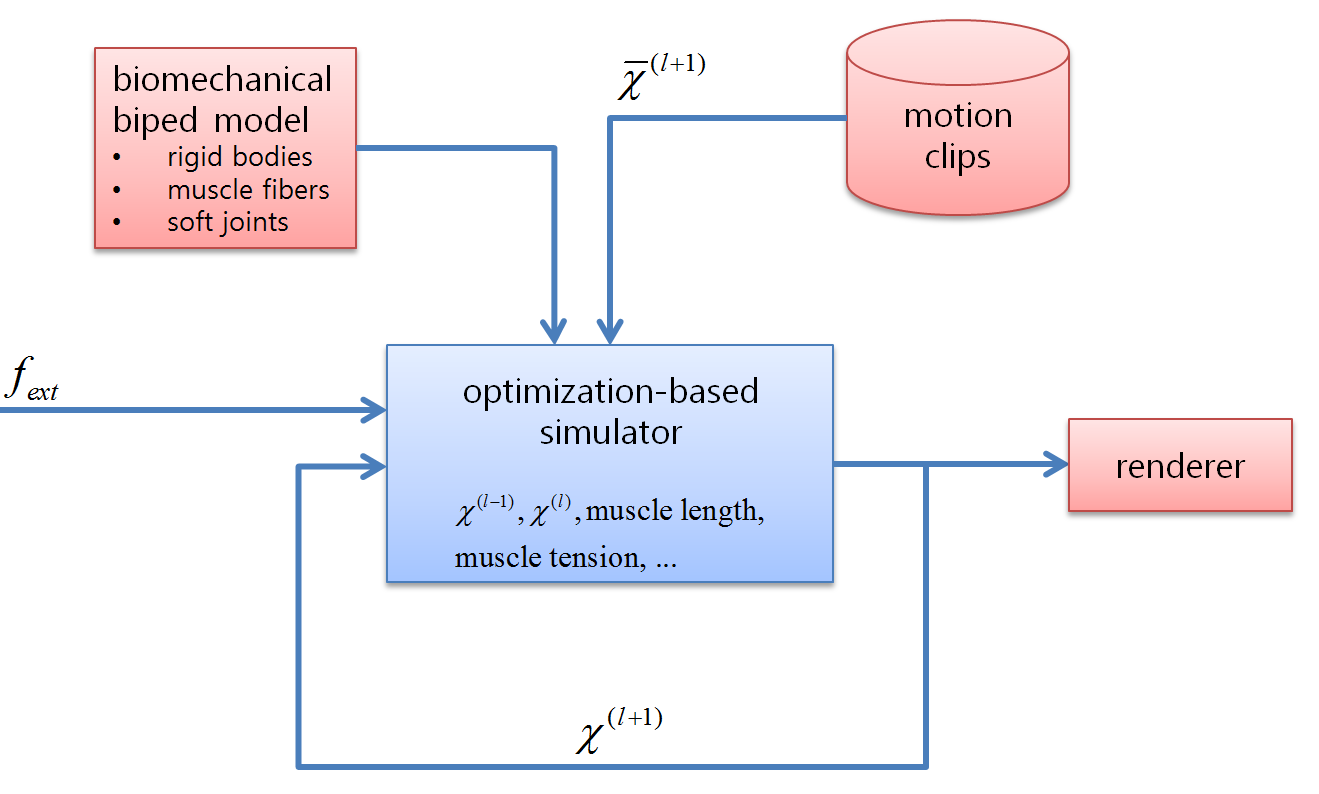
\includegraphics[width=0.75\textwidth]{overview2}
  \caption{Simulation outline}
  \label{overview2}
\end{figure}

This thesis is organized as follows. Chapter 2 describes related work,
focused on physically-based character animation and biomechanics model.
In Chapter 3 we will describe more details on our biomechanical biped simulation system
including muscle fiber model, soft joint model.
A reference tracking controller based on an optimization
using this biped model is presented in Chapter 4.
Results of tracking simulation is presented in Chapter 5,
and conclude with Chapter 6.

\chapter{Related work}

\section{Physically-based character animation}
Designing and controlling a physically simulated character is a long-standing
challenge in robotics and computer graphics. A physically
synthesized motion that actively responds to the environment is quite
promising because it is hard to keyframing a natural animation for every motion
manually. Although the combination of motion capture data and manual keyframing
shows a quality of motion, it is not straightforward to make a character
interacts with its environment if a pre-recorded motion clip is used.
By combining  a character animation system with physical simulation we can handle
this issue. The problem is that still there is no ultimate solution for controlling
a simulated character motion.

Some approaches proposed a controller which is based on the fact
that the ground reaction forces or contact forces affect the global
DOFs of the character significantly \cite{SCA07:249-258:2007, journals/tog/MuicoLPP09}.
Muico and his colleagues
presented a contact-aware controller \cite{journals/tog/MuicoLPP09}.
The approach is
heavily based on the theory of optimal control \cite{lewis}.
They modified the linear quadratic regulator (LQR) to consider the presence of the ground reaction forces.
We also take the contact forces into account but in a different way.
We estimate contact forces using a penalty-based method and an optimization framework
takes it into account for calculating actuation forces.

Using an optimization technique for biped control is relatively complicated method.
There exists a simpler way to control. KangKang Yin and her colleagues
presented a proportional-derivative (PD) control framework \cite{journals/tog/YinLP07}.
They used a finite state machine (FSM) in which target poses are defined
for each state. Considering the complexity of biped dynamics model,
the structure of controller is simple and robust to external disturbances.
Since they do not consider energy efficiency or passive forces during
control, the animation shows some stiff behavior.
Even if we can get more elaborate animations by increasing
the number of states in the FSM, it is not practically possible since the
number of parameters is proportional to the number of states.

Optimization-based approaches shown to be a good way to address many challenges
in biped control such as high dimensionality, underactuated-ness and
nonlinearity. Most of work set up their goal to determine the joint
torques to make a desired pose or a sequence of desired poses.
Instead of finding joint torques, Jain and his colleagues formulated
an optimization problem which finds joint angles directly \cite{Jain:09:OIM}. The joint torques
are implicitly calculated during the optimization process. The advantage of
this approach is that it is easy to design various types of objectives such as
moving a hand to nearby wall or placing a swing foot to a certain place while it
is not intuitive to formulate with torque-based optimization techniques.
We take a similar form except that we finds rigid body position
and orientation rather than joint angles during optimization.

%------%
\section{Biomechanical model}

Our work is related to literatures in biomechanics field.
Some researchers in biomechanical engineering focus on the movement
disorder and biomedical applications such as artificial joints.
There are abundant work exist which use a model similar to
a real human body since it is important to study the mechanism of underlying
structure of human body in such field \cite{vr-305}.

Thelen and his colleagues illustrated
an algorithm to compute muscle excitation patterns that produce
coordinated movements of muscle-actuated dynamic models \cite{Thelen2003321}.
They simulated
a pedaling motion of a person on a bicycle while fixing the upper body to investigate the excitation
pattern of 30 muscle fibers on both legs which significantly affecting the leg movements.

An anatomy-based approach for muscle animation is presented by Dong and his colleagues \cite{10.1109/2945.998668}.
They deal with the problem to muscle modeling that attempts to provide models for human musculature based
on the real morphological structures. Their main focus lies on visualizing muscle form and action in
great details.

Liu and her colleagues tried to exploit the passive characteristics of
real muscle fiber by including a torsion spring in joints \cite{Liu:2005:LPB}.
However, the actuation
is still occurred by joint motors and a musculoskeletal structure is not mentioned at all.

On the other hand, Lee and his colleagues accurately modeled human muscles on the upper body
to simulate the physics-based deformations of the soft tissues \cite{Lee:2009:CBM:1559755.1559756}.
They also designed an animation controller that computes the muscle activation signals to follow target poses
specified by an animator. Their model is heavily focused on realistic musculoskeletal
system and skin deformations for upper body.
Note that we present a simplified biomechanical biped model for synthesizing character animation,
not for visualizing or rendering skin deformation.

Lastly, human musculoskeletal structure is mainly referred from an article on Wikipedia \cite{Wikipedia},
Google Body Browser~\cite{bodybrowser} and a textbook written by Martini~\cite{martini}.
Also a well-known mathematical model of muscle fiber
called a Hill-type model is used in our model \cite{hill, Lee:2006:HUB:1141911.1142013}.


%The action for each muscle groups can be anticipated by adopting the
%fact regarding to gait phases \cite{perry}. The gait phases are the essential component
%when analyzing a person's walking pattern. It directly identifies the
%functional significance of the different motions occurring at the
%individual joints. While controlling the character we
%can determine the current gait phase. For each gait phase,
%a subset of the entire muscle fibers is selected to be actuated
%and the others will be unactuated.

%The muscle fiber model we use is composed of two springs and a damper.
%This simple muscle model is explained in detail in the supplementary
%documents [SHADMEHR]. In the document they assume that spring stiffness constants
%and viscosity of the damper are constants. Some studies suggest that animals
%vary stiffness according to the specific locomotion task.[FARLEY]
%Since the model consists of springs we definitely need rest lengths for that
%springs. However rest lengths are not simply defined on real muscles.
%[...]


\chapter{Biomechanical biped system model}

\section{Overview}

Modeling a precise and realistic human musculoskeletal structure for physics simulation
is challenging problem because there are enormous number of muscles and bones in human body.
Besides, their features, shapes, structures vary in wide range and it is hard to
model them accurately.
Our main interest lies on how to design a biped actuated by skeletal muscles with reasonable
simplification and assumption that is suitable for character animation.
Skeletal muscles on human body are depicted in Figure \ref{skelmus1} and \ref{skelmus2}.

\begin{figure}[h!]
  \centering
  \includegraphics[width=3.5in]{muscles_anterior_labeled}
  \caption{Human skeletal muscles (anterior)}
  \label{skelmus1}
\end{figure}

\begin{figure}[h!]
  \centering
  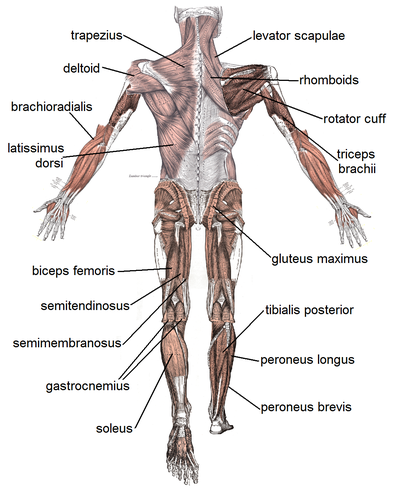
\includegraphics[width=3.5in]{Muscle_posterior_labeled}
  \caption{Human skeletal muscles (posterior)}
  \label{skelmus2}
\end{figure}
\noindent
A single muscle fiber is not acting alone as you can see in these figures.
So each tagged item does not indicate a muscle fiber, but a muscle body or muscle group.
A group of individual muscle fibers forms a muscle body (or simply muscle).
One or more muscles may be grouped by their similarity in features, and we call them a muscle group.
However, we will use terms muscles and muscle groups interchangeably.

Note that not all muscles in these figures are modeled into our model.
We focus on muscles related to legs which mainly contributes to locomotion
such as sartorius, gluteus maximus, quadriceps and so on.
Muscles used in our biped are listed in Table \ref{musclelist}.

\begin{table}[h!]
\centering
  \begin{tabular}{lccl}
  name                            &  origin       &insertion& action \\
  \hline
  gluteus maximus                 &               &         & abduct thigh\\
  gluteus medius                  &  1b           & 2b      & abduct thigh\\
  semimembranosus                 &  13a          & 8b      & flex knee \\
  semitendinosus                  &  11b          & 7b      & flex knee \\
  biceps femoris (long head)      &  14b          & 3b      & flex knee \\
  biceps femoris (short head)     &  14b          & 5b      & flex knee \\
  sartorius                       &  1a           & 10a     & flex thigh \\
  adductor longus                 &  3a           & 5a      & adduct thigh \\
  adductor magnus                 &  12b          & 10b,15b & adduct thigh \\
  gracilis                        &  3a           & 9a      & adduct thigh, flex knee \\
  rectus femoris                  &  2a           & 7a      & extend knee, flex thigh \\
  vastus medialis                 &  5a           & 8a      & extend knee \\
  vastus lateralis                &  4a           & 6a      & extend knee\\
  gastrocnemius                   &  4b, 9b       & 6b      & plantar flex foot, flex knee\\
  \hline
\end{tabular}
\caption[Muscles on a leg used in our model]
{Muscles on a leg used in our model: The location of origin and insertion
is described in Figure~\ref{fig:musclepoints} (a) and (b). For instance, the origin of
sartorius is located at mark 1 on Figure~\ref{fig:musclepoints} (a).}
\label{musclelist}
\end{table}

\begin{figure}[h!]
  \centering
  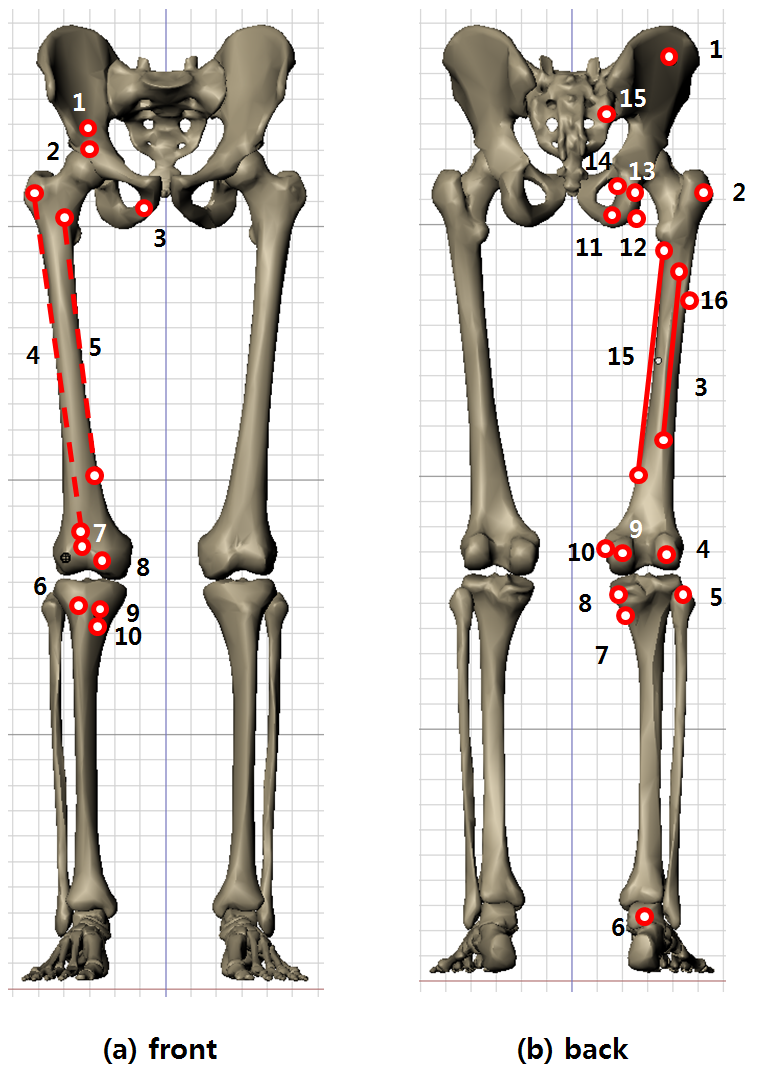
\includegraphics[width=4.8in]{musclepoints}
  \caption[Biomechanical modeling of a biped]
  {Biomechanical modeling of a biped: (a) and (b) depict origin and insertion points.
  The dashed lines in (a) denote lines at the back of the femur.
  (c) shows that body segments are modeled as rigid bodies.
   }
   \label{fig:musclepoints}
\end{figure}

Not all biological and anatomical facts and features about human muscles are considered.
We need some assumptions to make modeling of biomechanical biped system tractable.

First, we assume that each muscle body is composed of a reasonably small number of muscle fibers.
For example, one end of biceps femoris is connected to upper part of femur and tuberosity of the ischium (heap).
The other end is connected to upper part of fibula. So we model
the muscle using two muscle fibers. One connecting femur and fibula and the other connecting
heap and fibula (Figure \ref{muscleabs} (a)).
When a muscle attached to a large area on bones, we can use multiple muscle fibers
gathered around in a certain area. For example,
quadriceps femoris connects tibial tuberosity (knee side of tibia)
and femur. This muscle's attached area on the femur is wide. In this case,
we use multiple muscle fibers to model the muscle (Figure \ref{muscleabs} (b)).

Second, in fact a muscle is actually a soft deformable body.
So muscles can be deformed freely
with respect to configurations of attached bones or other reasons. It matters
in the case of doing skin deformations or accurate surgery simulation. However, in our model,
a muscle fiber is treated as a piston, both ends are rigidly connected to bones (modeled as rigid bodies)
through the form of ball joints. This is depicted in Figure \ref{muscleabs} (c) and (d).
In fact, we do not have any components deal with deformation.

Third, a detailed bone geometry is not considered on joints.
For example, a hip joint is formed by the articulation of the rounded head of the femur and
the cup-like acetabulum of the pelvis. Instead of modeling each skeleton's exact shape,
we use a box-shaped rigid bodies for representing body segments and assume bones lies
in the rigid bodies.

Fourth, some bones are removed or merged into other bones for simplicity.
Definitely, we do not need to model every fingers or toes with individual bones.
There are two bones called tibia and fibula on each calf.
However, we removed fibula because its feature is lost in humans~\cite{nofibula}.
Patella bones are omitted and we assumed that it is fixed on knee side of femur.

We model a body segment as a rigid body. One or more bones in human skeleton are
wrapped with a rigid body as shown in Figure~\ref{fig:musclepoints} (c).
We use a head-arm-trunk (HAT) model to focus on human locomotion.


\begin{figure}[h!]
  \centering
  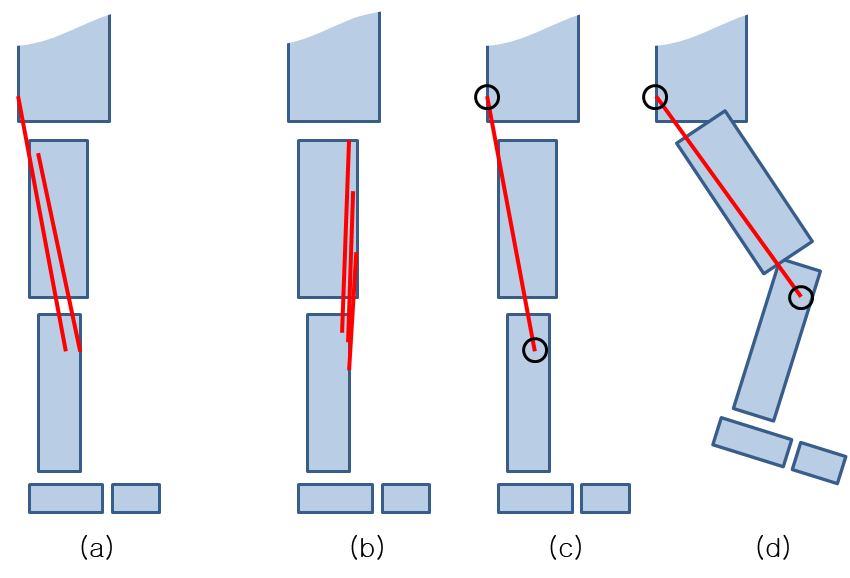
\includegraphics[width=3.5in]{muscleabs}
  \caption[Musculoskeletal modeling of a biped]{Musculoskeletal modeling of a biped:
  An anatomical figure between (a) and (b) shows muscles on right thigh.
  Red and green muscles indicate biceps femoris and quadriceps femoris, respectively. Black circles on
  (c) and (d) denote ball joints connecting both ends of the muscle to bones.}
  \label{muscleabs}
\end{figure}




\begin{table}[h!]
\centering
  \begin{tabular}{cccccc}
  name       &  full name                      &  origin       & insertion    & a1     &  a2 \\
  \hline
  SOL        & soleus                          &               & \\
  FLEXDIG    & flexor digit. longus            &               & \\
  FLEXHAL    & flexor hallis. longus           &               & \\
  TIBANT     & anterior tibialis               &               & \\
  EXTDIG     & extensor digit. longus          &               & \\
  EXTHAL     & extensor halli. longus          &               & \\
  VASINT     & vastus intermedius              &               & \\
  GMAX       & gluteus maximus ? (upper/lower) &               & \\
  ILIACUS    & iliacus                         &               & \\
  GMED       & gluteus medius                  &  1b           & 2b           & LR \\
  SEMIMEM    & semimembranosis                 &  13a          & 8b           & TS \\
  SEMITEN    & semitendenosis                  &  11b          & 7b           & TS \\
  BIFEMLH    & biceps femoris (long head)      &  14b          & 3b           & TS \\
  BIFEMSH    & biceps femoris (short head)     &  14b          & 5b           &        & IS\\
  SAR        & satorius                        &  1a           & 10a          &        & IS\\
  RF         & rectus femoris                  &  2a           & 7a           &        & PS\\
  ADDLONG    & adductor longus                 &  3a           & 5a           &        & PS\\
  AMAG       & adductor magnus                 &  12b          & 10b,15b      & TS,LR\\
  GRA        & gracilis                        &  3a           & 9a           &        & IS\\
  GMAX       & gluteus maximus ? (upper/lower) &               &              & LR\\
  ILIACUS    & iliacus                         &               &              &        & IS\\
  VASMED     & vastus medialis                 &  5a           & 8a           & LR \\
  VASINT     & vastus intermedius              &               &              & LR \\
  VASLAT     & vastus lateralis                &  4a           & 6a           & LR \\
  MEDGAS     & gastrocnemius (?)               &  4b, 9b       & 6b           & TST\\
  SOL        & soleus                          &               &              & TST\\
  FLEXDIG    & flexor digit. longus            &               &              & TST\\
  FLEXHAL    & flexor hallis. longus           &               &              & TST\\
  TIBANT     & anterior tibialis               &               &              & TS      & IS \\
  EXTDIG     & extensor digit. longus          &               &              &         & IS \\
  EXTHAL     & extensor halli. longus          &               &              &         & IS \\
  \hline
\end{tabular}
\caption{Muscles on a leg used in our model}
\label{muslist}
\end{table}


\begin{table}[h!]
\centering
  \begin{tabular}{cccccc}
  name       &  full name                      &  origin       & insertion    & a1     &  a2 \\
  GMIN       & gluteus minimus                 &               &              &    \\
  PERBREV    & peroneus brevis                 &  \\
  PERLONG    & peroneus longus                 &  \\
  HAMSTRINGS &                                 &  \\
  ADDBREV    &                                 &  \\
  TFL        &                                 &  \\
  PECT       &                                 &  \\
  PSOAS      &                                 &  \\
  QUADFEM    &                                 &  \\
  GLEM       &                                 &  \\
  PERI       &                                 &  \\
  LATGAS     &                                 &  \\
  SOLSTIF    &                                 &  \\
  TIBPOST    &                                 &  \\
  PERTERT    &                                 &  \\
  LIGPAT     &                                 &  \\
  TPOST      &                                 &  \\

  \hline
\end{tabular}
\caption{Muscles on a leg used in our model}
\label{muslist}
\end{table}

\begin{table}[h!]
\centering
  \begin{tabular}{cl}
  terminology         &  description \\
  \hline
  abduction           & move a limb away from the central line of the body \\
  adduction           & move a limb back toward, or even through, the central line of the body \\
  extension           & increase the angle between two bones, moving them away from each other \\
  flexion             & decrease the angle between two bones, bringing them together \\
  subtalar inversion  & faces the foot sole medially at the subtalar joint \\
  subtalar eversion   & faces the foot sole laterally at the subtalar joint \\
  plantar flexion     & points the toe to the ground at the ankle joint \\
  dorsi flexion       & lifts the foot up at the ankle joint \\
  rotation            & bone turns about its long axis \\
\end{tabular}
\caption{Terminology used in joint motion}
\label{termjointmot}
\end{table}


%Our character model is a full four-limbed biped, which consists of 14 rigid bodies.
%The list of rigid bodies with their configurations is given in Table \ref{bipedconf}.

%Mass of each body segment is referenced from \cite{humanbodydynamics}.
%We assume a uniform mass distribution for each rigid body.
%Length of each body is calculated from the skeleton configuration of motion capture data~\cite{cmumocap}.
%Other dimension is chosen arbitrarily.

%\begin{table}[h!]
%\centering
%  \begin{tabular}{crrl}
%                                                         & Name      & Mass $(kg)$  & Dimension $(m \times m \times m)$  \\
%  \hline
%  \multirow{8}{*}{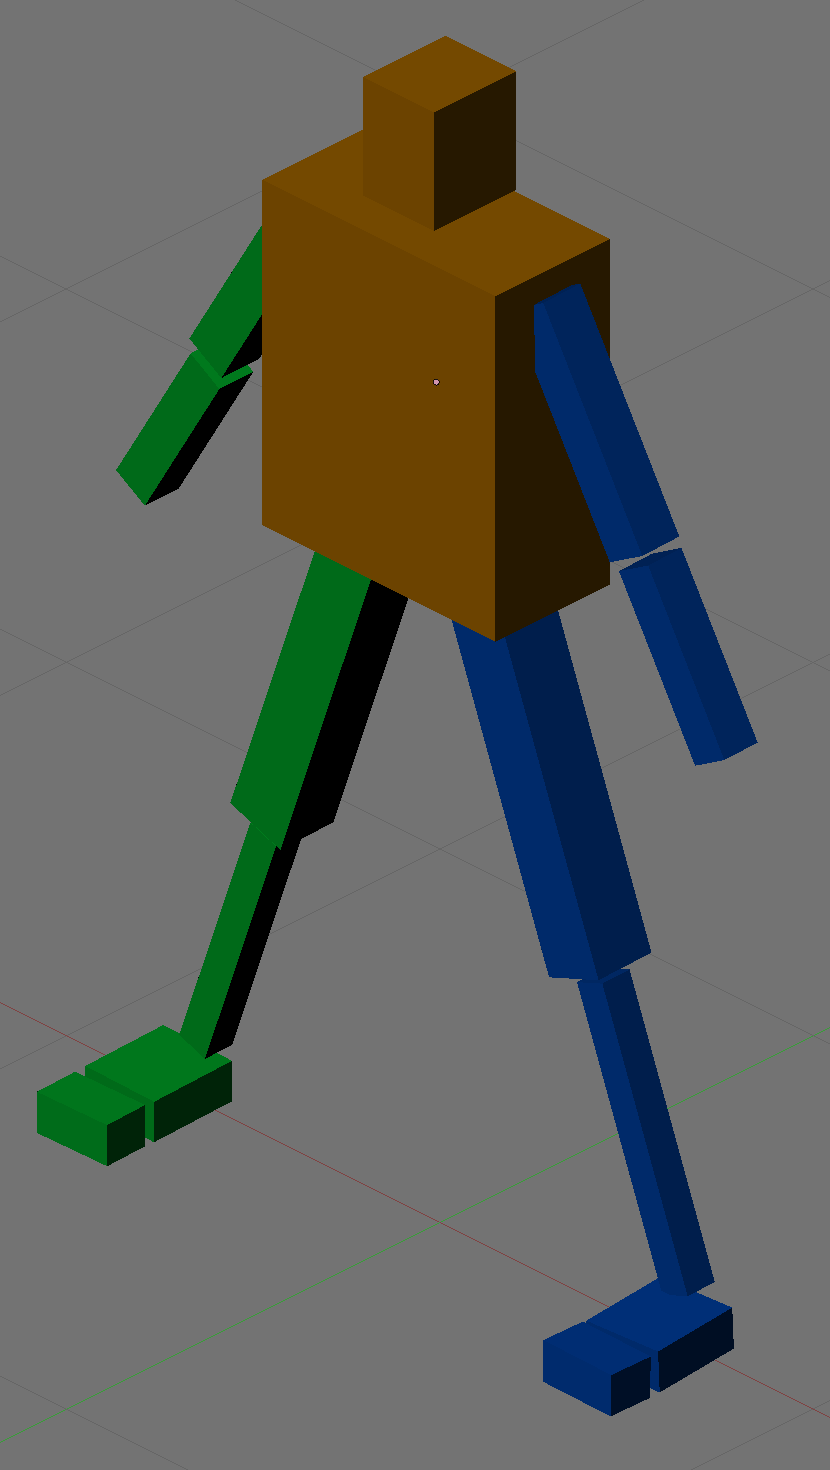
\includegraphics[width=0.85in]{biped}} & head      & 4.3          & $0.190 \times 0.220 \times 0.180$  \\
%                                                         & trunk     & 29.0         & $0.623 \times 0.507 \times 0.307$  \\
%                                                         & calf      & 2.7          & $0.073 \times 0.450 \times 0.073$  \\
%                                                         & thigh     & 6.3          & $0.142 \times 0.643 \times 0.142$  \\
%                                                         & sole      & 0.7          & $0.184 \times 0.210 \times 0.090$  \\
%                                                         & toe       & 0.2          & $0.184 \times 0.105 \times 0.090$  \\
%                                                         & upper arm & 2.0          & $0.100 \times 0.520 \times 0.100$  \\
%                                                         & lower arm & 1.1          & $0.090 \times 0.400 \times 0.090$  \\
%  \hline
%\end{tabular}
%\caption{Biped configuration}
%\label{bipedconf}
%\end{table}


\section{Muscle fiber model}

There are many variants of muscle fiber model used in biomechanical field range
from a simple time-invariant spring model to a complicated time-varying model \cite{25733}.
Although a more sophisticated model gives us a more realistic behavior, unnecessarily
complicated models will make the biped hard to simulate and control.
For a compromise, we use one of the simplest time-invariant spring-damper model commonly called
a Hill-type muscle model \cite{hill}. This model is depicted in Figure \ref{hilltype}

\begin{figure}[h!]
  \centering
  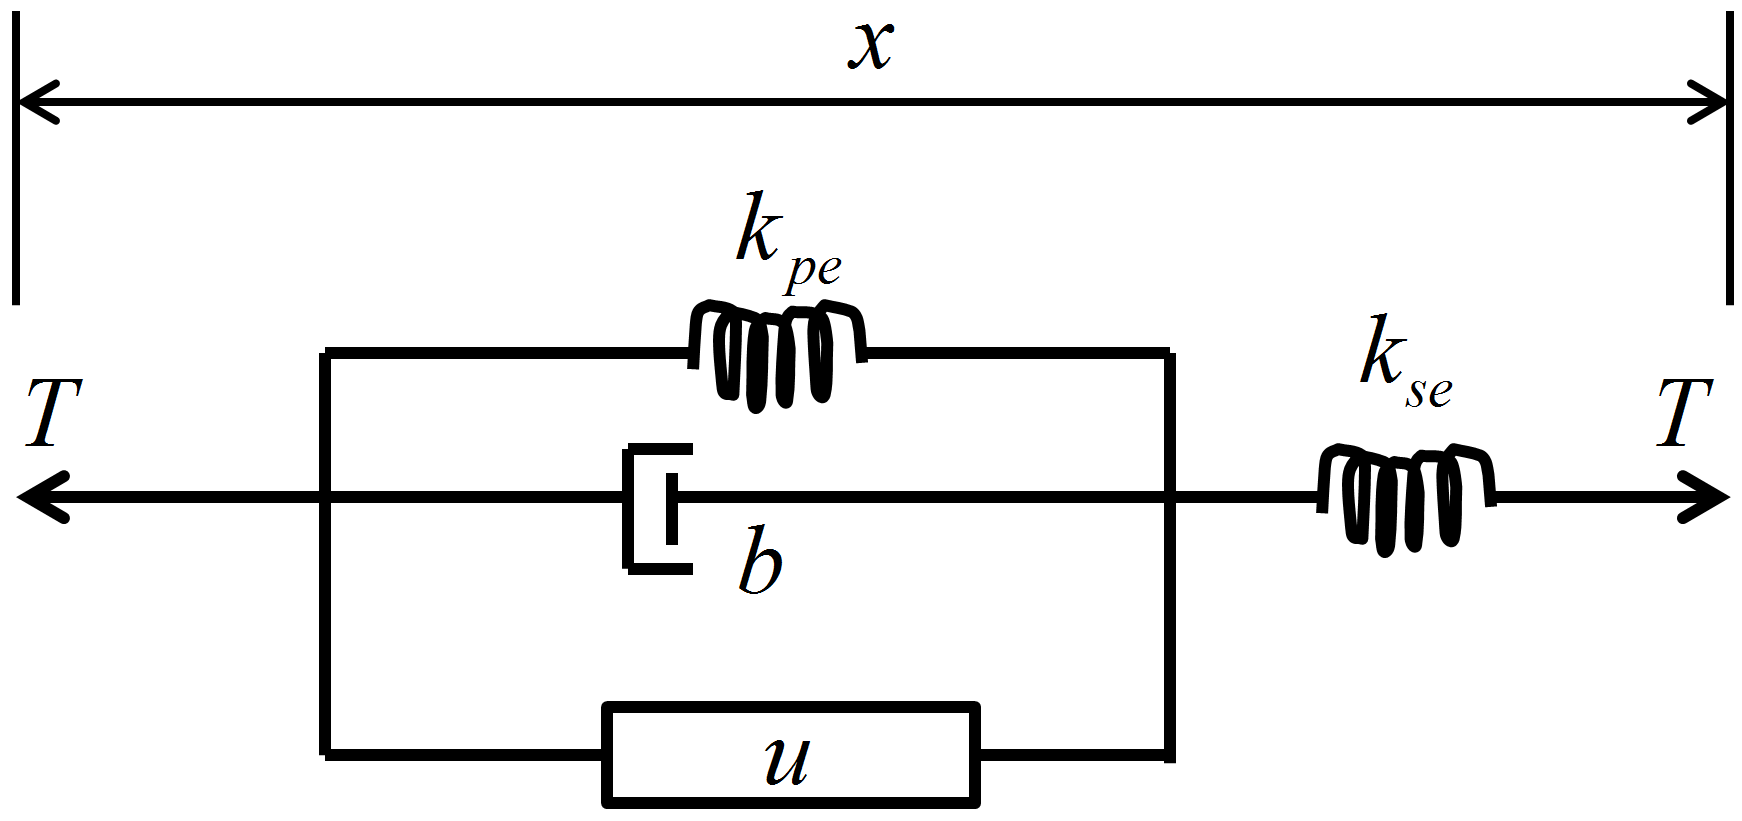
\includegraphics[width=2.6in]{musclemodel}
  \caption{Hill type muscle model}
  \label{hilltype}
\end{figure}
\noindent Basically, the model consists of two springs, a viscous damper and an uniaxial actuation component.
The damper and one of the springs are connected in parallel and the other spring is
connected in serial.
In real human body, many muscle fibers form bundles called \textit{fascicles}.
And multiple fascicles form a muscle body.
To simplify our biped model, we model a muscle body as a set of muscle fibers.
In the Hill-type muscle model, we need four parameters for each:
a serial spring constant $k_{se}$, a parallel spring constant $k_{pe}$, a viscosity $b$ and a rest length $x_{r}$.
These parameters can be constants or variables depending on how muscle fibers modeled.
A mathematical expression defining dynamics of the muscle fiber is a first-order ordinary differential equation:
\begin{equation}\label{Tension}
\dot{T} = \frac{k_{se}}{b} \left( k_{pe}(x-x_{r})+b\dot{x}-\left(1+\frac{k_{pe}}{k_{se}}\right)T+u   \right)
\end{equation}
where $T$ is a tension exerted at both ends (positive means pulling),
$x$ is the length of the fiber and $u$ is actuation force in the active component.
Note that all quantities shown in the equation are scalar values.
Each muscle fiber always connects two different rigid bodies and the same amount of
tension is applied to both of them with opposite directions.

Equation \eqref{Tension} can be transformed to a discretized version as done in equations of motion \eqref{MoEq2}.
Therefore, we can denote $T^{(l+1)}$ as a linear function of $T^{(l)}$, $x^{(l+1)}$, and so forth.

There are muscle terminology to clearly define the configuration of muscles.
A muscle fiber has an $origin$ and an $insertion$ which indicate the attached position
of various muscle fibers at certain bones.
In other words, an origin and an insertion refer where a muscle fiber is originated from and inserted to, respectively.
If we denote the origin and insertion position of the fiber as $p_{org}$ and $p_{ins}$ defined in
local Cartesian coordinates of respective body,
the normalized direction of the fiber can be defined as
$\hat{d}^{W}=(p^{W}_{ins}-p^{W}_{org})/||p^{W}_{ins}-p^{W}_{org}||$ where
a superscript $W$ means its position defined in world coordinates.
Thus, we can calculate tensions $T\hat{d}^{W}$ and $-T\hat{d}^{W}$.
These two forces are applied to the origin and the insertion body of the fiber, respectively (Figure \ref{orgins}).

There are such cases when fiber length becomes zero or near zero during simulation.
In that case, we assume that $d^{W}$ can be chosen arbitrarily
since the muscle direction is not well-defined.

\begin{figure}[h!]
  \centering
  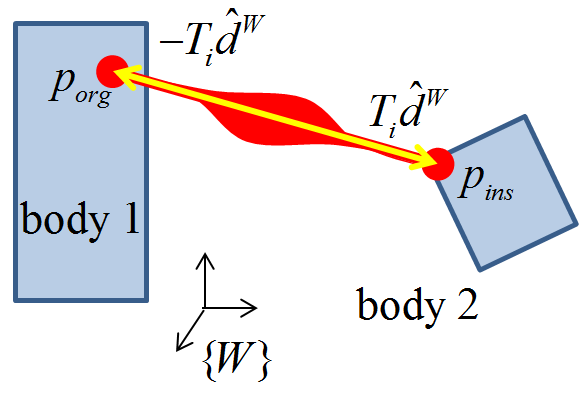
\includegraphics[width=1.8in]{orgins}
  \caption{Configuration of a muscle fiber attached to two rigid bodies}
  \label{orgins}
\end{figure}


We use two types of muscle fibers: actuated and unactuated muscle fibers.
Actuated muscle fibers represent the muscles we can actuate.
Ligaments keep joints in shape are modeled as unactuated muscle fibers.
Typically it is attached around joints. We cannot intentionally actuate unactuated muscle fibers.
Their purpose is to maintain its rest length to prevent joint dislocation.
For this reason, spring constants for unactuated fibers are comparatively larger than
the actuated muscle fiber values.

%An \emph{agonist}, or \emph{prime mover}, is a muscle whose contraction is chiefly responsible for producing a particular movement.
%A muscle fibers has its \emph{antagonist}. The antagonist is a muscle whose action opposes that of a particular agonist.
%We can choose specific muscle fibers to be used in the biped model based on agonists related to legs.
%Also we can inform the optimizer to reduce actuation force on a muscle fiber when its antagonist is actively actuated.

\section{Soft joints}

Conventional biped models use reduced coordinates to represent a pose.
This is possible because DOFs on rigid bodies are reduced by connecting them with
joints. They use 6-DOF on the root of the biped, \emph{i.e.} pelvis, for position and orientation.
The other rigid bodies except the root have three or less DOFs with respect to joint types and
typically do not have position (translation) part at all.
This implies that joint dislocation is impossible to occur
using conventional biped models.

On the contrary, every body segment in the biped model we propose has a full 6-DOF
to allow a joint dislocation.
In dynamics point of view, multiple rigid bodies are simulated individually
without any joint constraints involved.
Without joint constraints, the shape of biped is not maintained well
due to a serious joint dislocation occurred during optimization process.
For instance, all bodies may collapse to the ground with their joints broken apart
instead of preserved in shape.
By all means a certain human pose should be maintained and this is critically
related to degrees of joint dislocation.

We introduce soft joints which prevent serious joint dislocation on our biped model.
A soft joint is defined using two points, $p_1$ and $p_2$, on local coordinates of two
different rigid bodies and a dislocation threshold $r$ (Figure~\ref{fig:softjoint}).
The distance between two points should be bounded to $r$.
We connect two points with a stiff ligament fiber which help to satisfy the constraint.

%With these kind of joints, the biped can take advantages of shock absorption
%mechanism as well as prevention of joint dislocation.

\begin{figure}[h!]
  \centering
  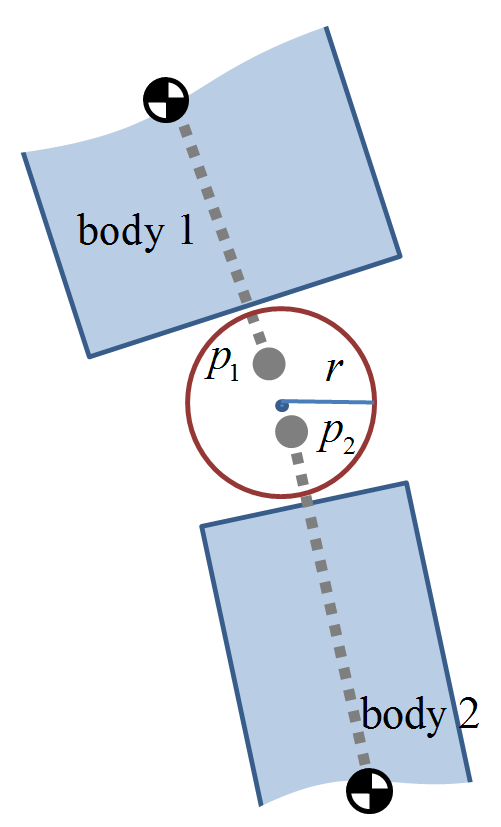
\includegraphics[width=1.3in]{softjoint}
  \caption{Structure of a soft joint}
  \label{fig:softjoint}
\end{figure}




\section{Gait phases}

Walking is a highly coordinated series of falls that we have taken for granted since we were toddlers.
%It takes 40 or so muscles just to raise one leg and move it forward.
In order to provide the basic functions required for walking, each stride
involves an ever-changing alignment between the body and the supporting foot during stance
and selective advancement of the limb segments in swing.
These reactions result in a series of motion patterns performed by the hip, knee and ankle.
The investigators of gait analysis found that each stride contains eight functional patterns~\cite{perry}.
We call these patterns \textit{gait phases}. Eight gait phases make a single \textit{gait cycle}.
Gait phases are listed on Table~\ref{gp}. Here we summarize the interval for each phase.

\begin{list}{\labelitemi}{\leftmargin=3em}
\setlength{\itemsep}{0cm}
\setlength{\parskip}{0cm}
\item {\bf initial contact (IC)}:
The limb is positioned to start stance with a heel.
\item {\bf loading response (LR)}:
The phase begins with initial floor contact and continues until the other foot is lifted for swing.
\item {\bf mid stance (MSt)}:
It begins as the other foot is lifted and continues until body weight is aligned over the forefoot.
\item {\bf terminal stance (TSt)}:
It begins with heel rise and continues until the other foot strikes the ground.
Throughout this phase body weight moves ahead of the forefoot.
\item {\bf pre-swing (PSw)}:
It begins with initial contact of the opposite limb and ends with toe-off.
\item {\bf initial swing (ISw)}:
It begins with lift of the foot from the floor and ends when the swinging foot is opposite the stance foot.
\item {\bf mid swing (MSw)}:
This phase begins as the swinging limb is opposite the stance limb.
The phase ends when the swinging limb is forward and the tibia is vertical.
\item {\bf terminal swing (TSw)}:
The final phase of swing begins with a vertical tibia and ends when the foot strikes the floor.
Limb advancement is completed as the leg (shank) moves ahead of the thigh.
\end{list}


Stride is the equivalent of a gait cycle. It is based on the actions of one limb.
The duration of a stride is the interval between two sequential initial floor contacts by the same limb.

For each gait phase, mainly activated muscles and their activation patterns are known.
We exploit this to control biped locomotion.

\begin{table}[h!]
\centering
  \begin{tabular}{ccccc}
          task                         &phase no. & name   &  full name        & contacted             \\
  \hline
  \multirow{2}{*}{weight acceptance}   & 1        &  IC    & initial contact   & no $\rightarrow$ yes  \\
                                       & 2        &  LR    & loading response  &      yes              \\
  \hline
  \multirow{3}{*}{single limb support} & 3        &  MSt   & mid stance        &      yes              \\
                                       & 4        &  TSt   & terminal stance   &      yes              \\
                                       & 5        &  PSw   & pre-swing         &      yes              \\
  \hline
  \multirow{3}{*}{limb advancement   } & 6        &  ISw   & initial swing     & yes  $\rightarrow$ no \\
                                       & 7        &  MSw   & mid swing         &       no              \\
                                       & 8        &  TSw   & terminal swing    &       no              \\
  \hline
\end{tabular}
\caption{Gait phases}
\label{gp}
\end{table}

\begin{figure}[h!]
  \centering
  \includegraphics[width=4in]{phase}
  \caption{Gait phases of two limbs}
  \label{fig:softjoint}
\end{figure}

\chapter{Physics simulation and optimization}

\section{Equations of motion}

Equations of motion governing the movement of rigid bodies can be written as follows:
\begin{equation}\label{MoEq2}
\mathbf{M}(\chi)\ddot\chi + C(\chi,\dot\chi )
 = f_g + f_c + f_f  + f_{ext} = f
\end{equation}
where $\mathbf{M}$ is a generalized mass matrix and $\chi$ is a generalized
linear and angular position
state vector and $\dot\chi$, $\ddot\chi$ are its first and second time derivatives,
respectively. $C$ represents Coriolis and centrifugal forces.
$f_c$ represents contact forces or ground reaction forces.
$f_f$ denotes muscle forces occurred from muscle fiber tensions.

For the case of a freely moving single
rigid body with 6-DOF with $n_f$ muscle fibers attached,
$\mathbf{M}$ will be $6\times 6$ matrix and $\chi$,
$C$, $f_g$, $f_c$ and $f_f$ will be a 6-dimensional vector. $f_f$ is the sum of
each muscle fibers forces, that is $\sum f_{f,i}$ where $i=1,\dots,n_f$.

Because we represent times as discrete samples, all the functions of
time-varying variables need to be represented in a discrete domain.
We discretize the time into samples with small intervals $h$. We define
the velocity $\dot\chi^{(l)}$ and the acceleration $\ddot\chi^{(l)}$, at current
time sample $l$, by backward and central finite differences, respectively.
\begin{align}
\dot\chi^{(l)}  \equiv {} & \frac{\chi^{(l)}-\chi^{(l-1)}}{h}\label{vel-dis}\\
\ddot\chi^{(l)} \equiv {} & \frac{\chi^{(l+1)}-2\chi^{(l)}+\chi^{(l-1)}}{h^2}\label{acc-dis}
\end{align}
By substituting \eqref{vel-dis} and \eqref{acc-dis} into \eqref{MoEq2},
we can denote $\chi^{(l+1)}$ as a linear function of $\chi^{(l)}$, $\chi^{(l-1)}$ and so forth.
Notice that we embedded Euler integration step into equations of motion by this substitution.

As stated in Chapter 1, most of the existing work on
character animation used an articulated body to represent a character.
In the articulated model, each body is connected to another body with
various types of joints such as hinge joints and ball joints.
Therefore, So called joint constraint equations additionally
needed for that model.
On the other hand, since we use no joint at all in the character
model, the equations of motion of the whole biped is just a independent collection of
\eqref{MoEq2}. This is shown in the following equation.

\begin{equation}
\left [
\begin{array}{ccc}
\mathbf{M}_1                      &            &                               \\
                                  &  \ddots    &                               \\
                                  &            & \mathbf{M}_{|\mathcal{B}|}    \\
\end{array}
\right ]
\left [
\begin{array}{c}
\ddot{\chi}_1 \\
\vdots \\
\ddot{\chi}_{|\mathcal{B}|}
\end{array}
\right ]
+
\left [
\begin{array}{c}
C_1 \\
\vdots \\
C_{|\mathcal{B}|}
\end{array}
\right ]
=
\left [
\begin{array}{c}
f_1 \\
\vdots \\
f_{|\mathcal{B}|}
\end{array}
\right ]
\end{equation}
Since this permits independent rigid body movements,
our model may allow joint dislocation.
We will introduce a concept of soft joints to prevent serious
joint dislocation in subsequent section.



\section{Contact model}

We use a penalty-based method which can be easily integrated in our optimization framework.
It estimates contact normal forces with allowing a certain amount of penetration.
A temporary spring-damper element is created and attached where a contact is established.
The spring-damper exerts a strong force to separate two penetrated bodies.
After non-penetration constraints recovered the spring-damper is removed immediately.
Typically, a critically-damped spring is used to make the separation time minimal without oscillation.

\begin{figure}[h!]
  \centering
  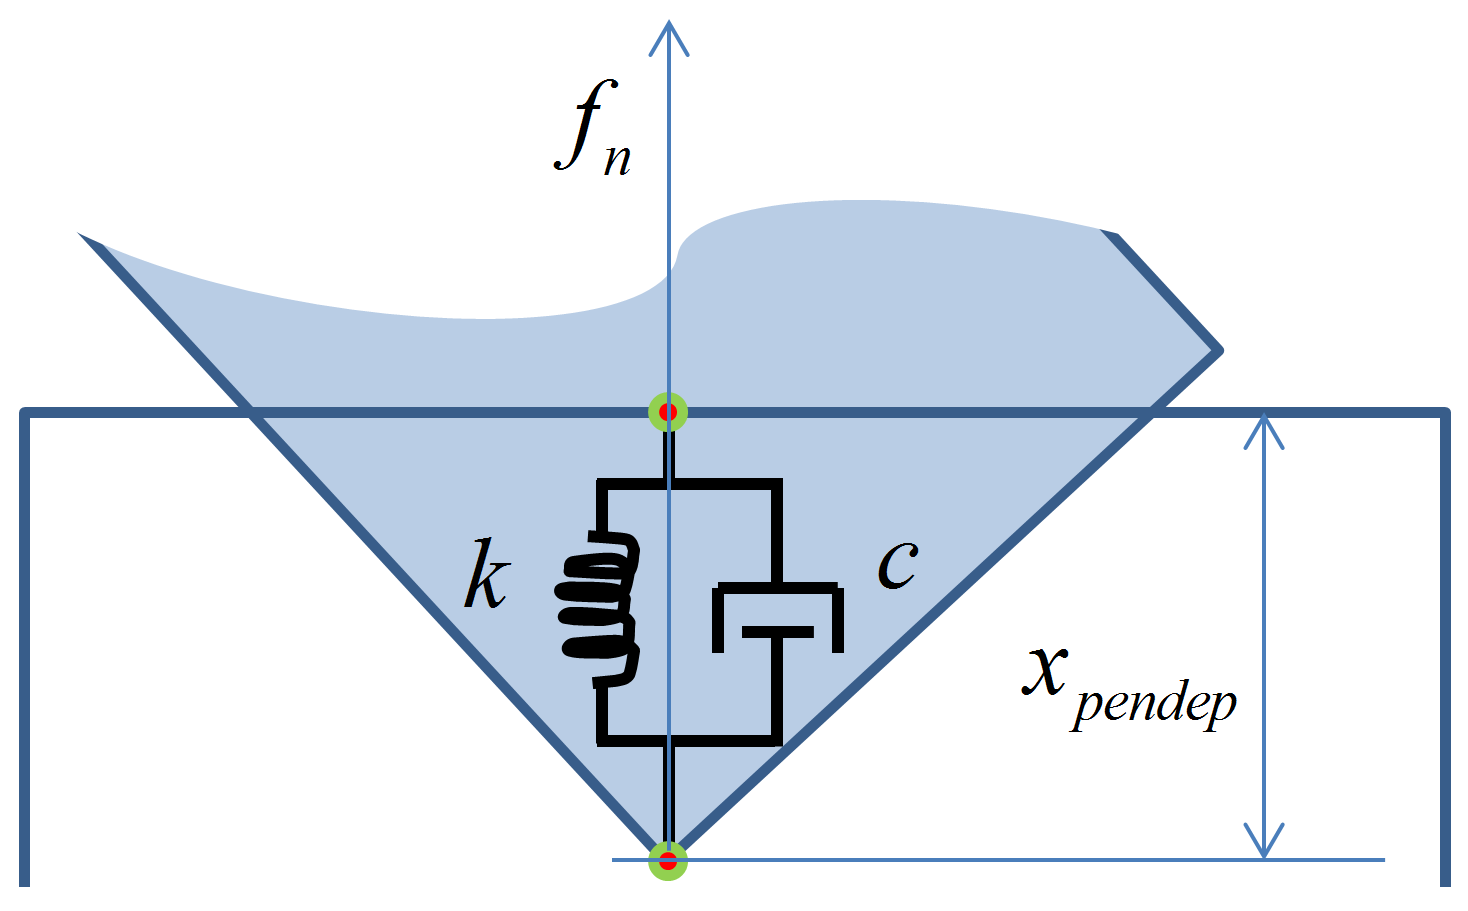
\includegraphics[width=2.0in]{penalty}
  \caption{Normal force calculated from the penalty method}
\end{figure}

Normal force exerted at the penetrated corner point of the box is calculated as follows:
\begin{equation}\label{penalty-normal}
f_n = -k x - c \dot{x}
\end{equation}
where $f_n$ is the normal force, $k$ is a spring constant, $c$ is a damping coefficient and $x$ is
a penetration depth. $k$ and $c$ is positive numbers and $x$ is a negative in case of penetration.
If a single rigid body of body mass $\bar{m}$ has $n_p$ contact points with the ground,
$n_p$ springs of the damping coefficient $c=2\sqrt{\bar{m}k/n_p}$ makes a critically damped system.

Since any normal force should be applied in unilateral manner, \emph{i.e.},
only pushing a penetrated body not pulling, we need an additional constraint $f_n \geq 0$.
$x$ will be always a negative scalar, so the term $-kx$ is always become a positive.
A problem arises when a penetrated corner point is in a separation phase,
especially when $kx < c\dot{x}$ which leads $f_n$ to a negative value.
To circumvent this issue, we add a nonnegative positive scalar term $\lambda$ to the right-hand side
of \eqref{penalty-normal} to obey the constraint $f_n \geq 0$. During optimization,
a minimal $\lambda$ to keep the constraint will be calculated
when we set a very high cost on that variable. We can denote \eqref{penalty-normal} with
discrete-time substitution that can be used as an equality constraint for the optimizer.
\begin{equation}\label{penalty-normal-discretized}
f_n = -k x^{(l+1)} - c \frac{x^{(l+1)} - x^{(l)}}{h} + \lambda
\end{equation}
Besides normal force, tangential contact force are needed to model friction.
Coulomb friction model is widely used.
There are two kinds of friction in this model: static friction and dynamic friction.
If contact points are sliding along the surface without breaking contacts,
dynamic friction force will act upon them. In this case, the friction force is depends
on the magnitude of normal force and velocity of sliding contact point along the surface.
Dynamic friction force $f_{tk}$ is
\begin{equation}\label{dynamic-friction}
f_{tk} = -\mu_k v |f_n|
\end{equation}
where $\mu_k$ is a coefficient of dynamic friction
and $v$ is velocity of sliding contact point along the surface.
On the other hand, a static friction force occurs on a stationary contact point.
In this case, a contact force should lies on a cone shaped geometry so-called
the Coulomb's friction cone. It is allowed to choose any static friction force as far as
the resulting contact force is in the cone.
We have two equations to express conditions of the static friction force:
\begin{equation}\label{static-friction}
\mu_s |f_n| \geq |f_{ts}|, \quad f_{ts} \cdot \hat{f}_n = 0
\end{equation}
where $f_{ts}$ is static friction force and $\mu_s$ is a coefficient of static friction.
Inner product equality implies that $f_{ts}$ should lies on the tangential space of contact point.



\section{Optimization}
So far, we described our biomechanical biped model as well as basic building blocks for rigid body dynamics
simulation.
Using this model, we design a tracking controller based on an optimization technique.
There are four types of constraints: equations of motion, muscle fiber tensions, contact forces and soft joints.
Equations of motion \eqref{MoEq2} govern motions of rigid bodies composing the biped.
Muscle fiber tensions cannot be chosen arbitrarily but should be calculated from the
discretized version of \eqref{Tension}
which is a linear function of actuation forces $u$, muscle fiber length $x$ and its rest length $x_r$.
Contact forces applied to the biped should conform \eqref{penalty-normal-discretized} and \eqref{static-friction} if
they are static or \eqref{penalty-normal-discretized} and \eqref{dynamic-friction} otherwise.
Lastly, soft joint constraints help to find the pose without serious joint dislocation.

\begin{equation}\notag
\text{minimize} \quad w_{ref} || \chi^{(l+1)} - \bar{\chi}^{(l+1)} || + w_u || u ||
\end{equation}
\begin{align}
\text{subject to} & \quad \chi^{(l+1)} = \tilde{\mathbf{M}}^{-1} (f_g + f_c + f_f + f_{ext} - \tilde{C})     &                      \notag\\
                  & \quad f_{f,i} = (-1)^{q} ( A_i u_i + B_i x_r + C_i ) d^W_i                      & i \in \mathcal{M}    \label{mf}\\
                  & \quad f_{c,i} = f_{n,i} + f_{tk, i}                                             & i \in \mathcal{P}_k  \notag\\
                  & \quad f_{c,i} = f_{n,i} + f_{ts, i}                                             & i \in \mathcal{P}_s  \notag\\
                  & \quad r_i \geq || Z_i \chi^{(l+1)} + V_i ||                                     & i \in \mathcal{J}    \label{sj}\\
                  & \quad u_{min}   \leq u   \leq u_{max}                                           &                      \notag\\
                  & \quad x_{r,min} \leq x_r \leq x_{r,max}                                         &                      \notag
\end{align}
A variable $q$ appeared in \eqref{mf} is 0 or 1
if tension is acting on origin body or insertion body, respectively.
$\mathcal{P}_k$ and $\mathcal{P}_s$ denote a set of dynamic contacts and a set of static contacts, respectively.
Please note that we omit some constraints such as Coulomb friction cone constraints \eqref{static-friction} for brevity.
In Equation \eqref{sj}, we estimate next step's joint anchor position in world coordinate.
Please refer to \cite{Jain:09:OIM} for detailed derivation.

The optimizer tries to find next pose $\chi^{(l+1)}$ which is as close as possible
to $\bar{\chi}^{(l+1)}$ with minimal efforts.
Optimization variables are $u$, $x_r$ and $f_{ts}$.
Solving the optimization problem is done for each simulation frame.
After next state $\chi^{(l+1)}$ is calculated, current state is updated to
next state and the frame counter $l$ is increased by 1.




\chapter{Results}


We used MOSEK optimization solver to solve
the optimization problem formulated in the previous chapter~\cite{mosek}.
We selected 17 muscles on legs and modeled them with about 300 muscle fibers.
The size of optimization problem is mainly
dependent on the number of rigid bodies, muscle fibers, soft joints
and contact points. Except contact points, every components
constituting a part of the biped is the same for the whole simulation process.
Therefore, runtime performance is slightly varied between frames
with respect to the number of contact points. In average, the solver takes
about 0.1 second for each frame. The ground spring constant $k=50000$ $N/m$ and
the time step $h=0.003$ $s$ are used.

There are a lot of parameters to decide especially in muscle fibers.
We tried to find Hill type muscle parameters for human, but there is no
such work providing them. Even though some work provide specific parameters,
but in crude manner. For example, a musculoskeletal dynamics system simulator
OpenSim uses a muscle model proposed by Schutte~\cite{Delp07}. But they used
the same damping coefficient regardless the type of muscle fibers.
Muscle rest lengths are determined from muscle lengths
when the biped stands straight. Other muscle parameters are summarized in Table \ref{musparm}.

\begin{table}[h!]
\centering
  \begin{tabular}{ccc}
            &  actuated muscles      &  unactuated muscles (ligaments) \\
  \hline
  $k_{se}$  &        10 $\sim$ 1000  &           1000                  \\
  $k_{pe}$  &        0.1 $\sim$ 10   &           0                     \\
  $b$       &        0.1             &           0.1                   \\
  \hline
\end{tabular}
\caption{Muscle fiber parameters}
\label{musparm}
\end{table}

The cost function of optimization plays a great role for tweaking
animation. For instance, if we suppress actuation force by increasing $w_u$
the biped will move limply. However, please note that arbitrary
weights are not always give you the proper motion sequence.

We used a straight walking motion sequence
for a reference trajectory. The snapshots of resulting motion is
shown in Figure \ref{fig:snapshot1} and \ref{fig:snapshot2}.
Deviation between reference trajectory and simulated motion is
depicted in Figure \ref{fig:devi}.

%Muscle fiber parameters can be varied to get different styles of motions.
%For example, a high $k_{se}$ gives more robot-like movement while a low value
%gives human-like elastic motion. However, viscous damping constant
%$b$ does not play a significant role in making various motions.

%Employing soft joints instead of rigid joints allows some limited
%dislocation. This leads to a better performance on tracking deviation.
%For example, let us assume that the biped extends its swing foot
%forward during tracking process. A contact time of swing foot with
%ground may differ from the reference trajectory
%and the simulated biped. By dislocating ankle, knee and hip joints
%a little, the contact time difference may be decreased.

%will affect every body segment because they are connected with
%one or more rigid joints. On the other hand, in our model,
%external force in a certain range on a body segment will only
%affect on that body by allowing a little dislocation on joints.

\begin{figure}
  \centering
  \subfloat{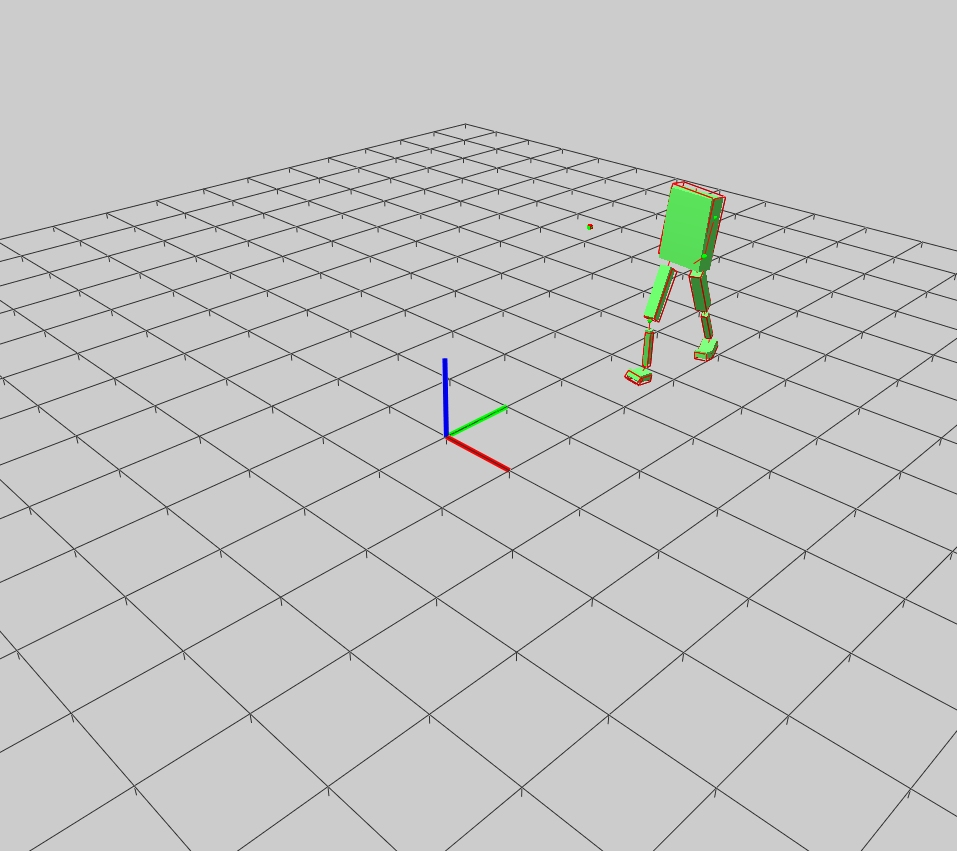
\includegraphics[width=1.5in]{pymss/00001}}
  \subfloat{\includegraphics[width=1.5in]{pymss/00021}}
  \subfloat{\includegraphics[width=1.5in]{pymss/00041}}
  \subfloat{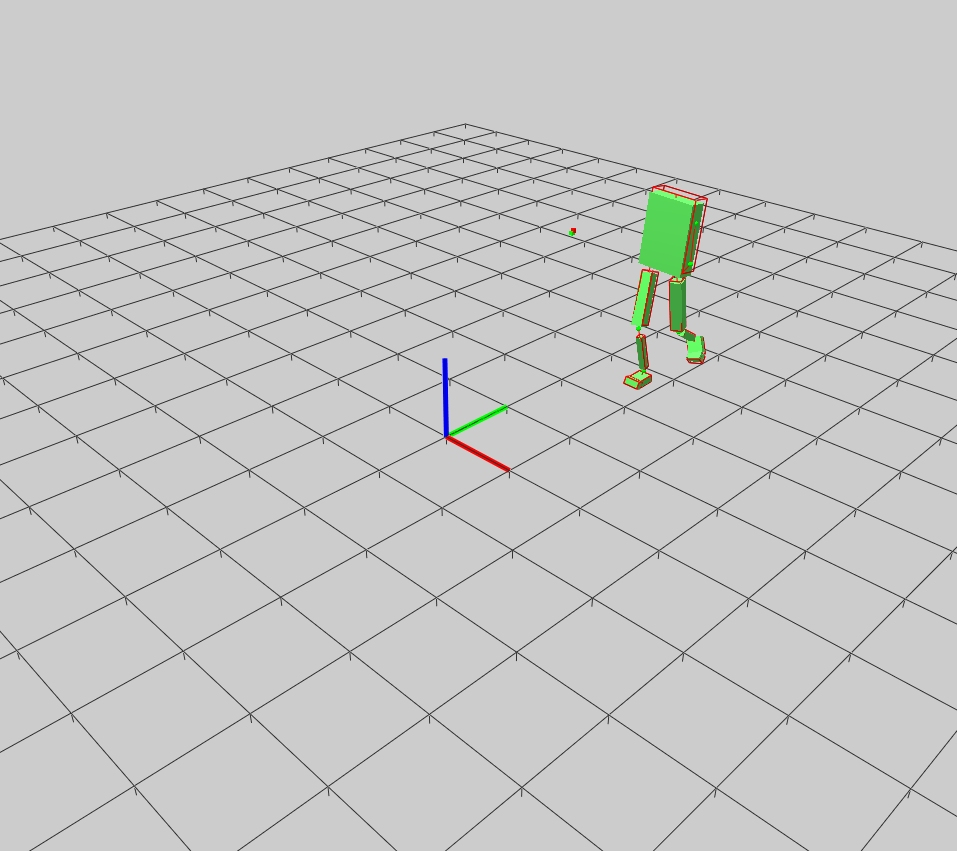
\includegraphics[width=1.5in]{pymss/00061}}\\
  \subfloat{\includegraphics[width=1.5in]{pymss/00081}}
  \subfloat{\includegraphics[width=1.5in]{pymss/00101}}
  \subfloat{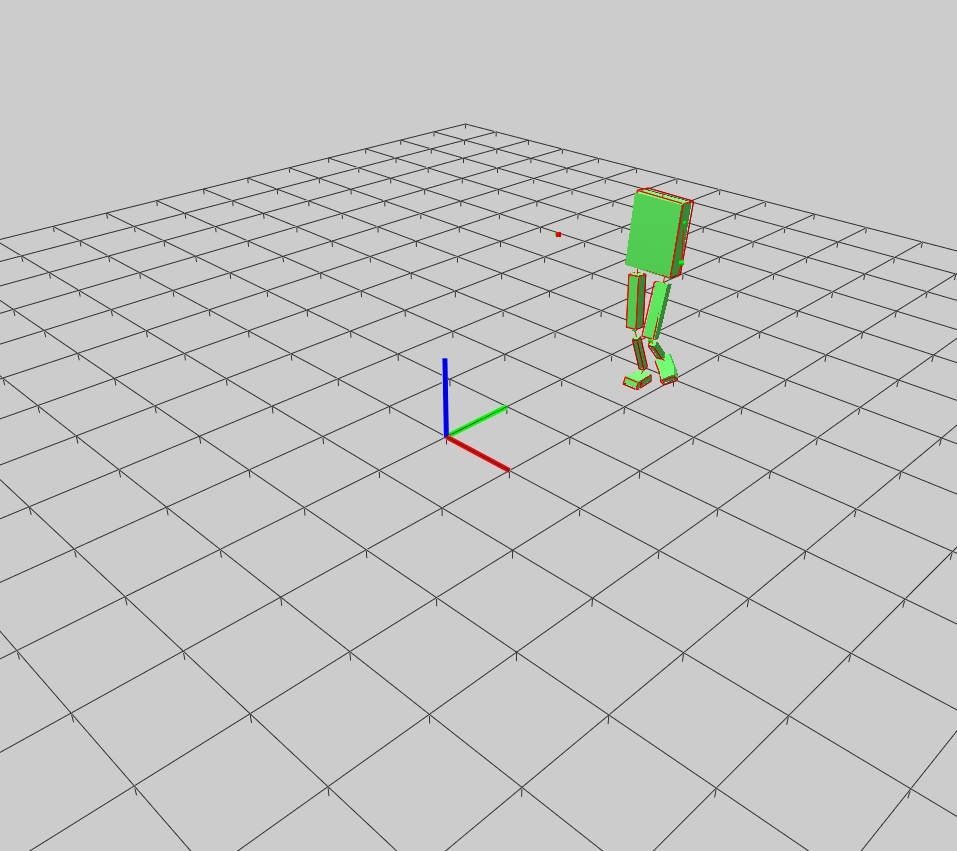
\includegraphics[width=1.5in]{pymss/00121}}
  \subfloat{\includegraphics[width=1.5in]{pymss/00141}}\\
  \subfloat{\includegraphics[width=1.5in]{pymss/00161}}
  \subfloat{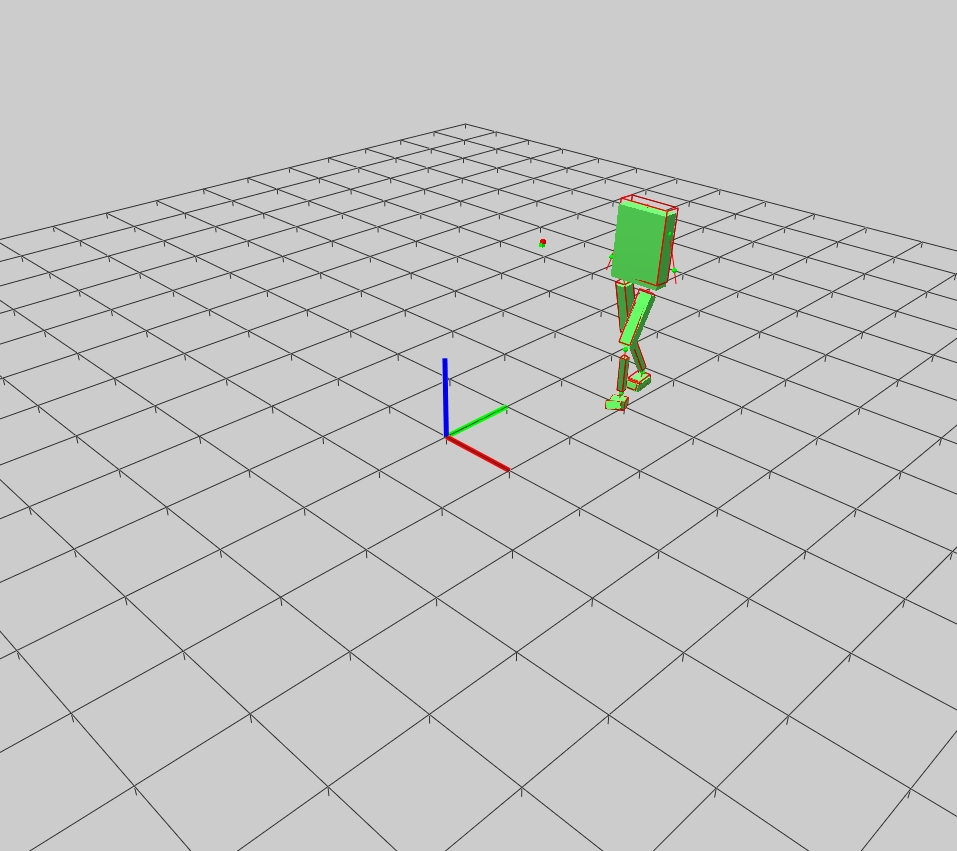
\includegraphics[width=1.5in]{pymss/00181}}
  \subfloat{\includegraphics[width=1.5in]{pymss/00201}}
  \subfloat{\includegraphics[width=1.5in]{pymss/00221}}\\
  \subfloat{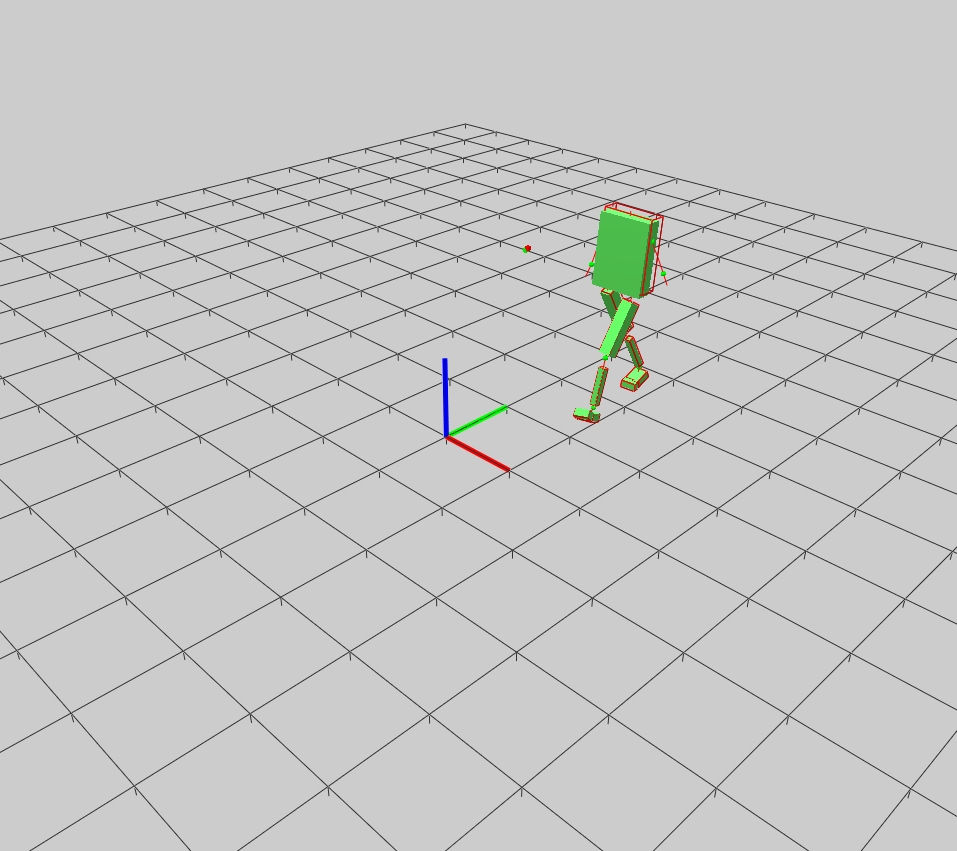
\includegraphics[width=1.5in]{pymss/00241}}
  \subfloat{\includegraphics[width=1.5in]{pymss/00261}}
  \subfloat{\includegraphics[width=1.5in]{pymss/00281}}
  \subfloat{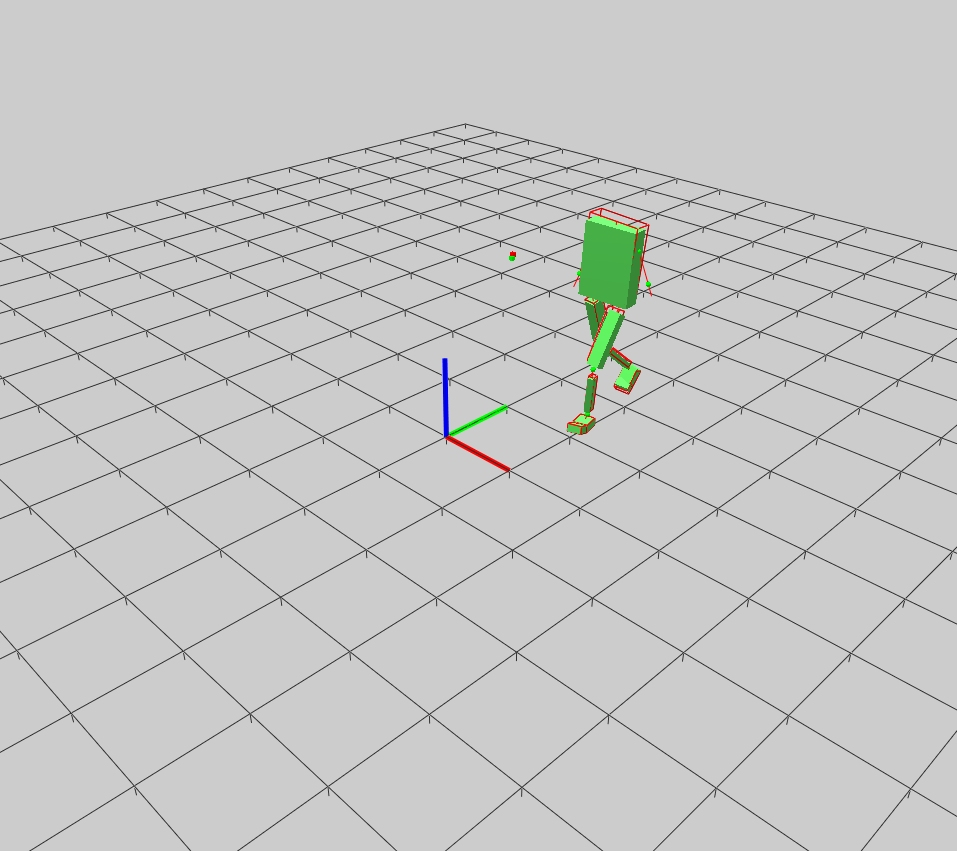
\includegraphics[width=1.5in]{pymss/00301}}\\
  \subfloat{\includegraphics[width=1.5in]{pymss/00321}}
  \subfloat{\includegraphics[width=1.5in]{pymss/00341}}
  \subfloat{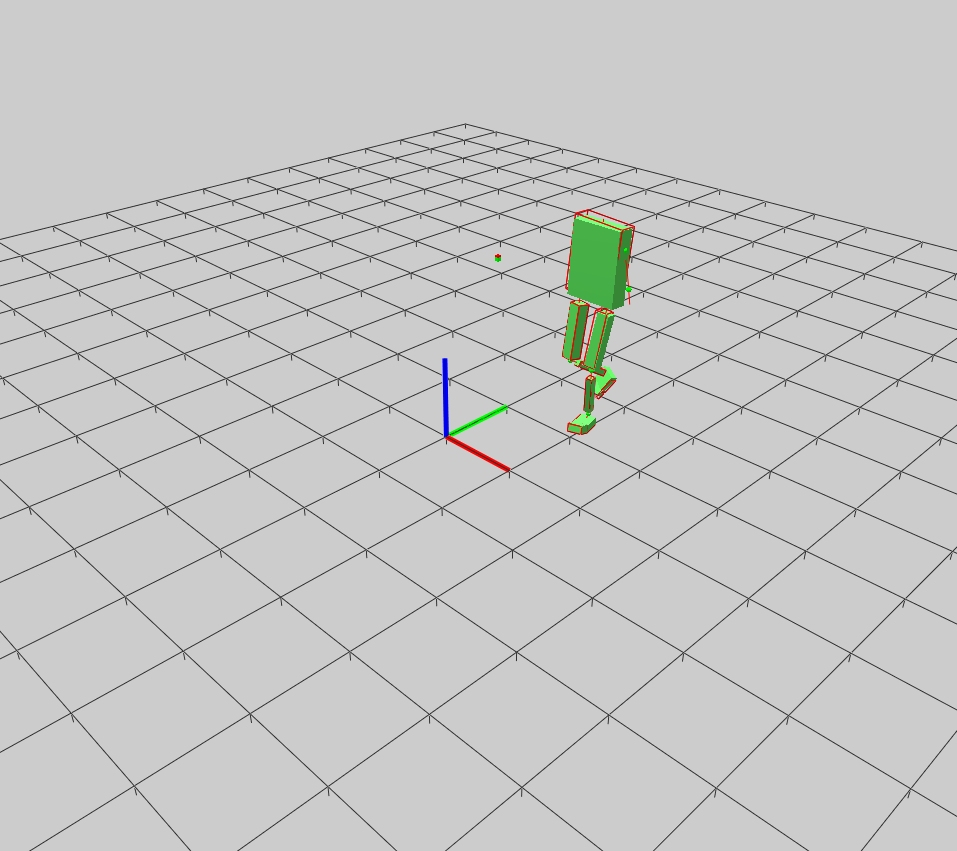
\includegraphics[width=1.5in]{pymss/00361}}
  \subfloat{\includegraphics[width=1.5in]{pymss/00381}}\\
  \caption{Locomotion snapshots (1 of 2)}
  \label{fig:snapshot1}
\end{figure}

\begin{figure}
  \centering
  \subfloat{\includegraphics[width=1.5in]{pymss/00401}}
  \subfloat{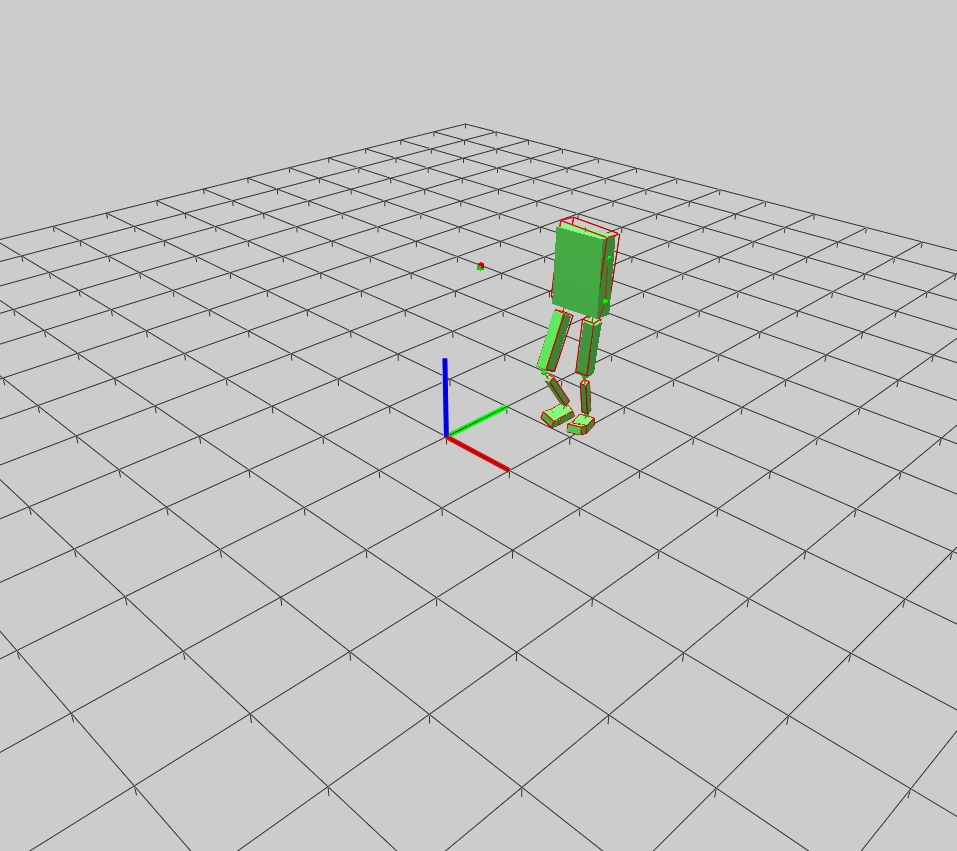
\includegraphics[width=1.5in]{pymss/00421}}
  \subfloat{\includegraphics[width=1.5in]{pymss/00441}}
  \subfloat{\includegraphics[width=1.5in]{pymss/00461}}\\
  \subfloat{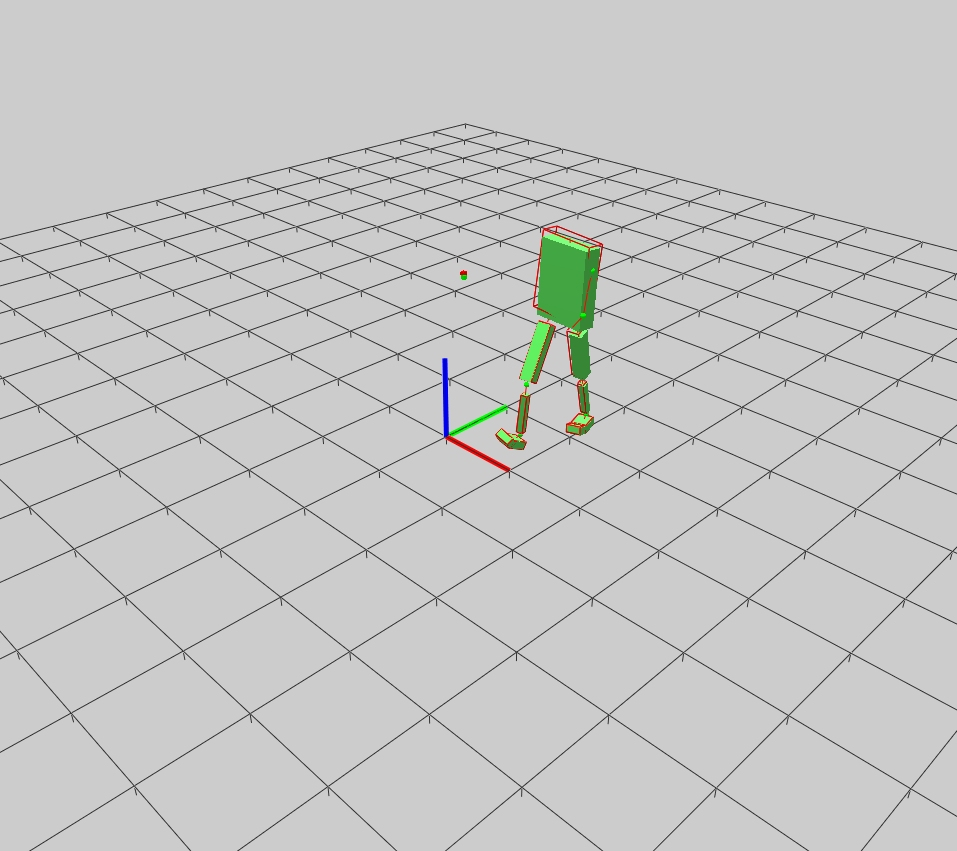
\includegraphics[width=1.5in]{pymss/00481}}
  \subfloat{\includegraphics[width=1.5in]{pymss/00501}}
  \subfloat{\includegraphics[width=1.5in]{pymss/00521}}
  \subfloat{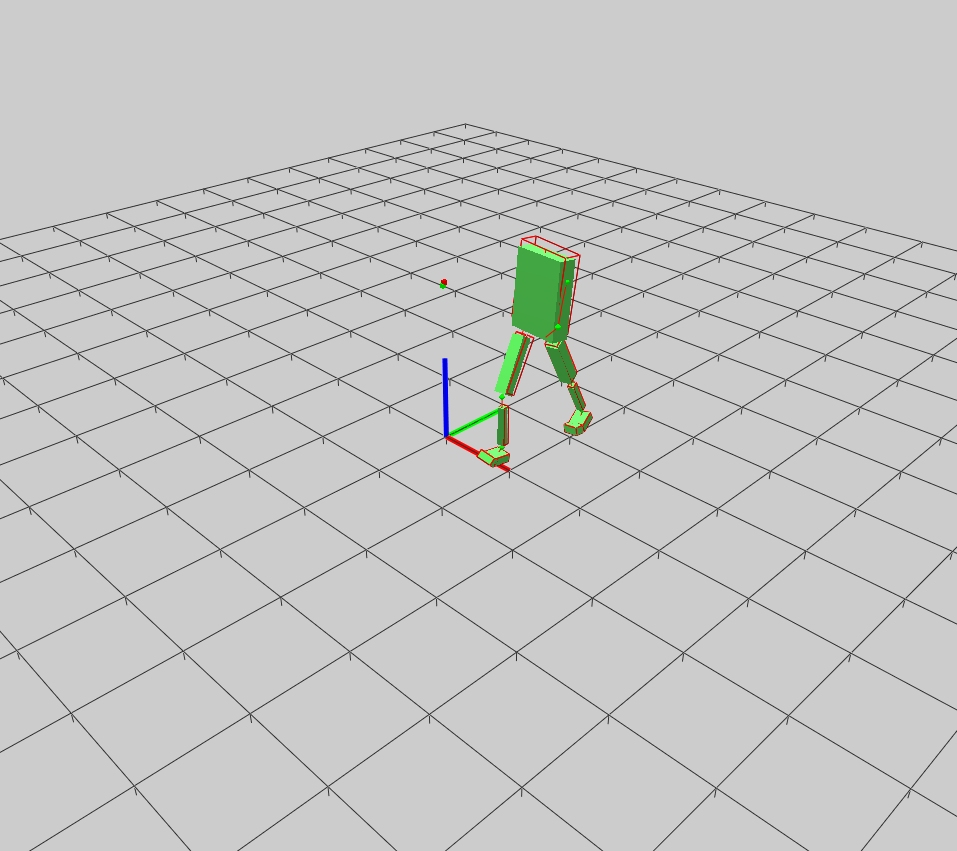
\includegraphics[width=1.5in]{pymss/00541}}\\
  \subfloat{\includegraphics[width=1.5in]{pymss/00561}}
  \subfloat{\includegraphics[width=1.5in]{pymss/00581}}
  \subfloat{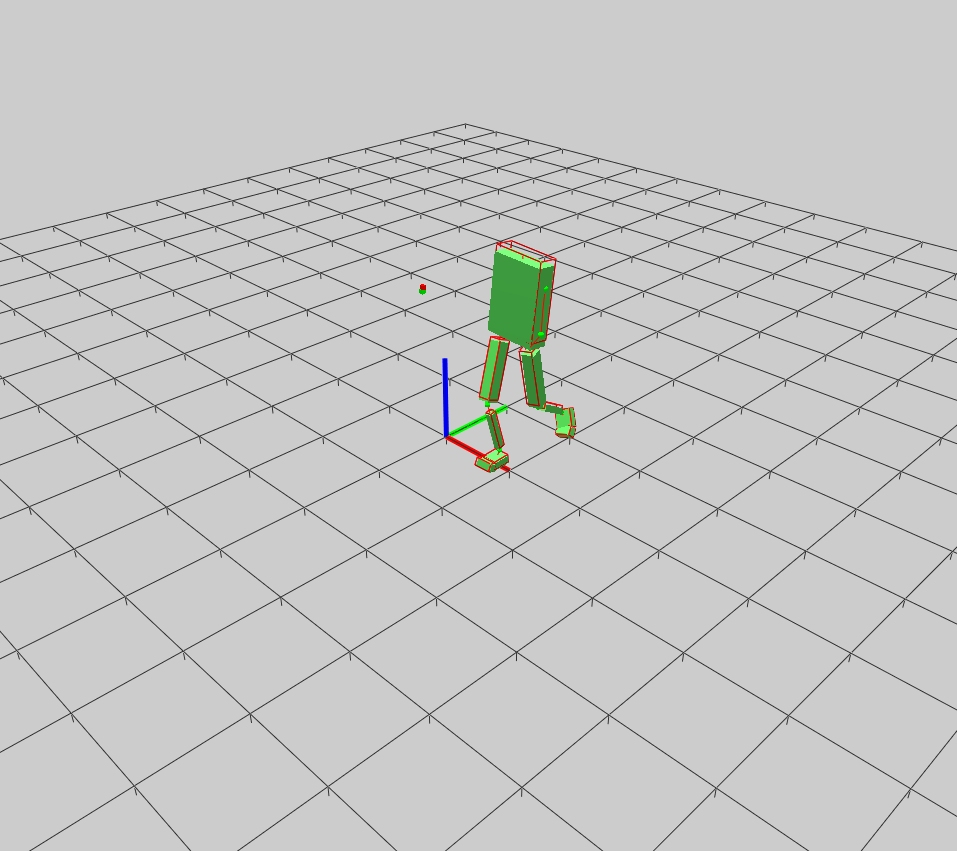
\includegraphics[width=1.5in]{pymss/00601}}
  \subfloat{\includegraphics[width=1.5in]{pymss/00621}}\\
  \subfloat{\includegraphics[width=1.5in]{pymss/00641}}
  \subfloat{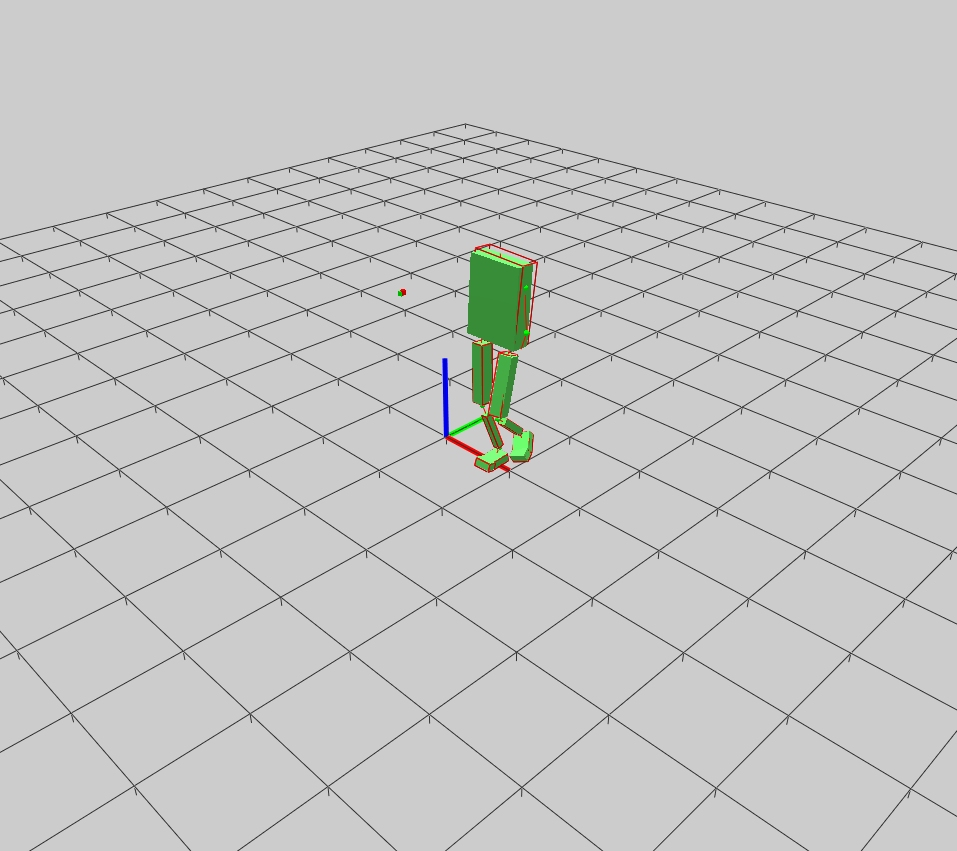
\includegraphics[width=1.5in]{pymss/00661}}
  \subfloat{\includegraphics[width=1.5in]{pymss/00681}}
  \subfloat{\includegraphics[width=1.5in]{pymss/00701}}\\
  \caption{Locomotion snapshots (1 of 2)}
  \label{fig:snapshot2}
\end{figure}

\begin{figure}[h!]
  \centering
  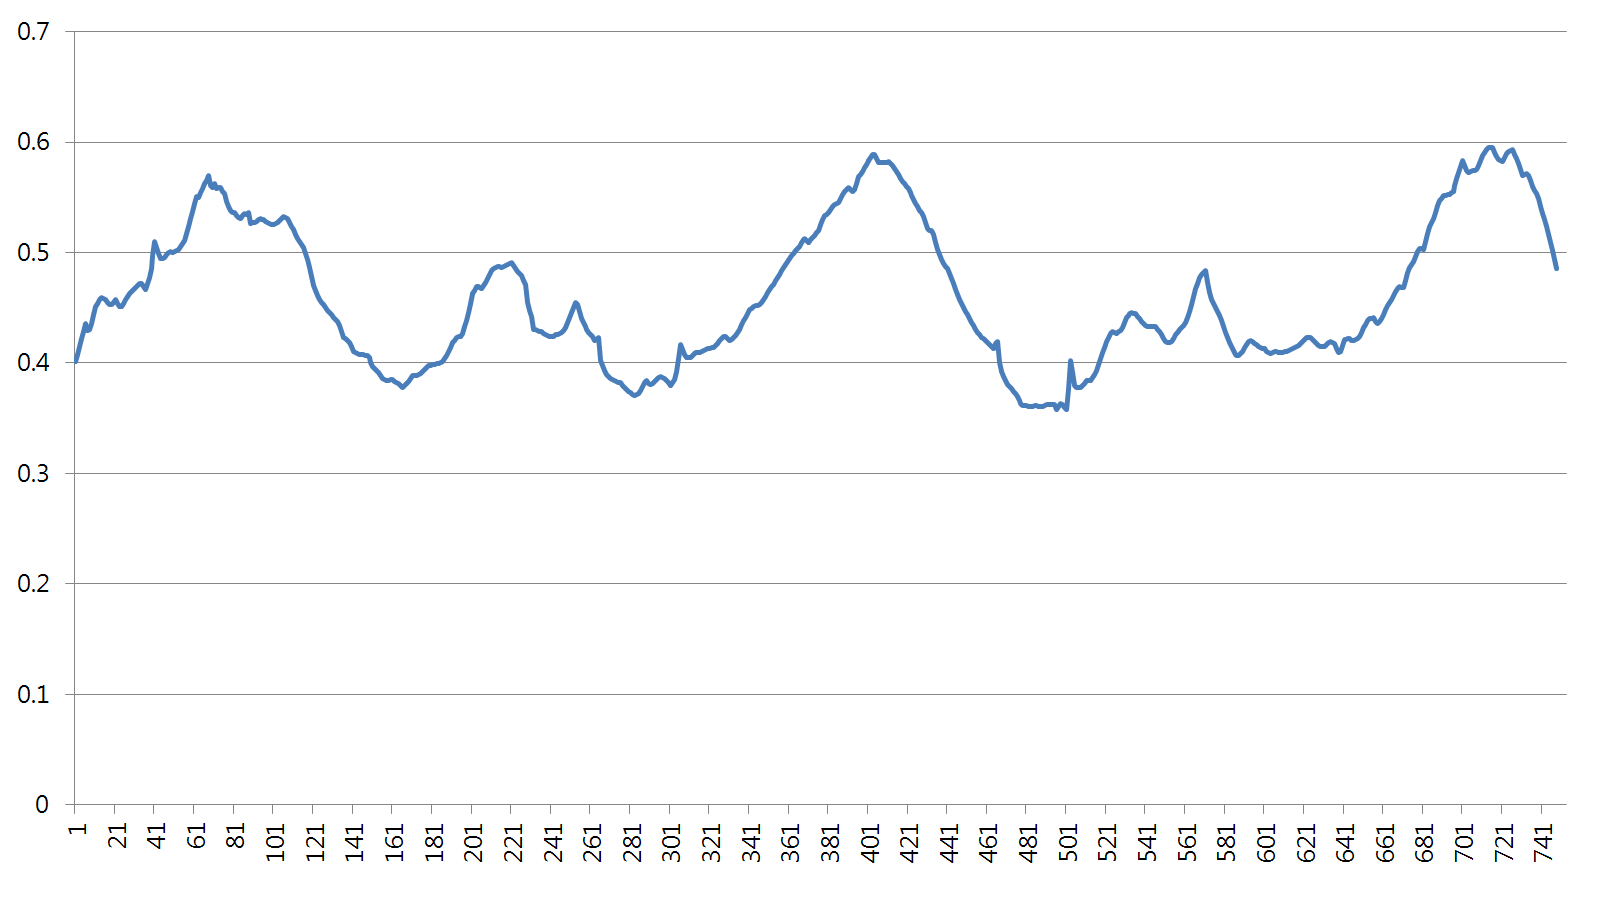
\includegraphics[width=5.in]{reftrack}
  \caption[Reference tracking performance]{Reference tracking performance: $x$-axis denotes the simulation frame index and $y$-axis denotes $||\chi-\bar{\chi}||$.}
  \label{fig:devi}
\end{figure}


%begin{figure}[h!]
% \centering
% 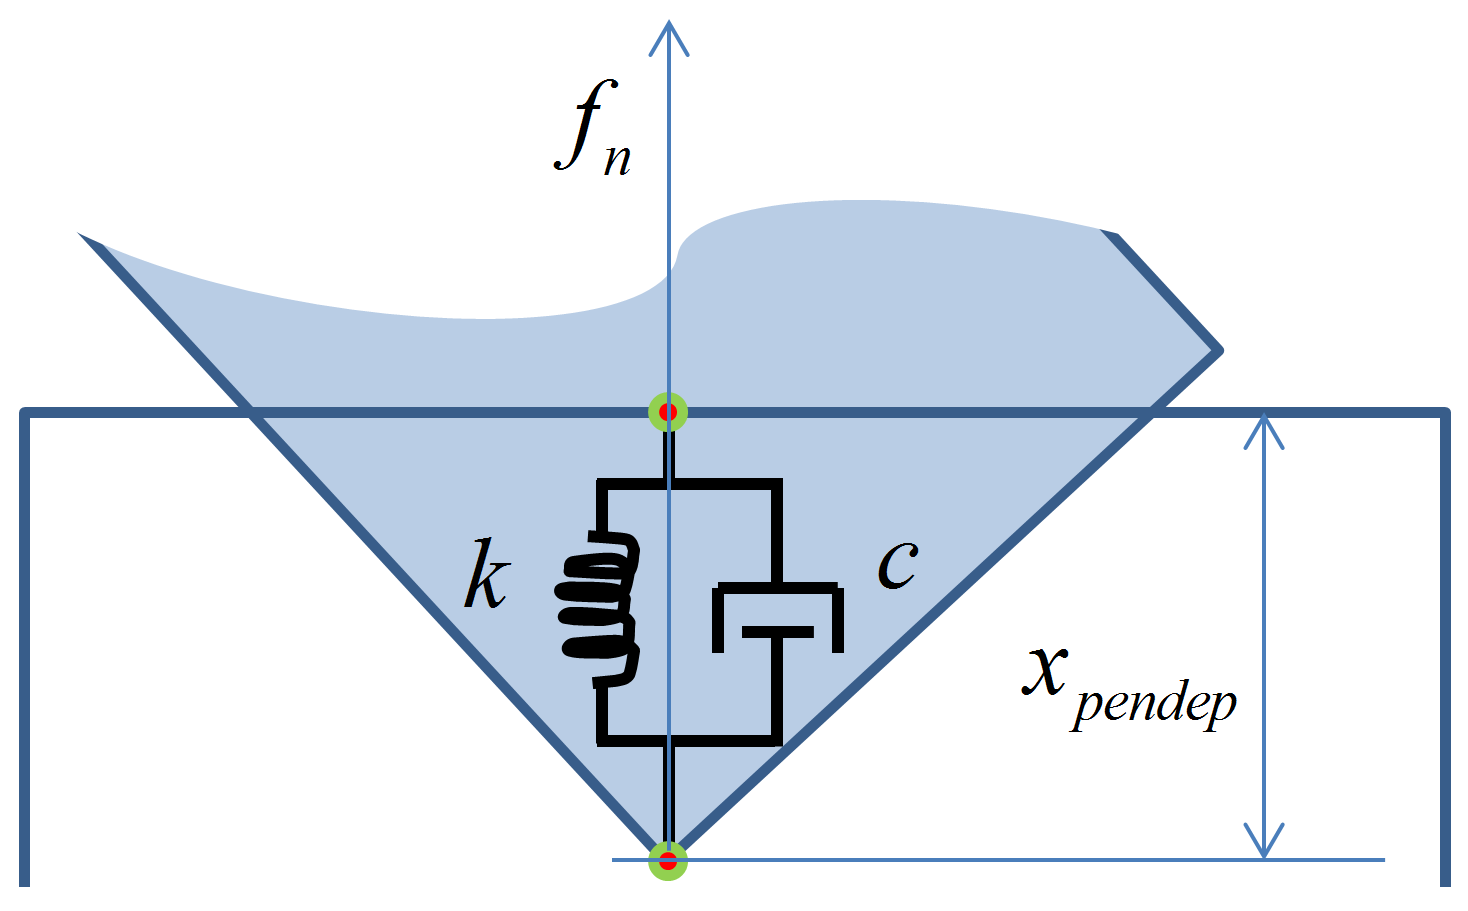
\includegraphics[width=2.0in]{penalty}
% \caption{Normal force calculated from the penalty method}
%end{figure}

\chapter{Conclusion}
In this thesis, we introduced a biomechanical biped model
which can be used for synthesizing character animation.
Muscle fibers are used to actuate rigid bodies instead of
joint motors. Soft joints used instead of conventional joints.
With our proposed model, we designed a locomotion controller
based on an optimization. There are some work related
to realistic human musculoskeletal system for visualization,
but none of them addresses an issue related to biped locomotion.
%human joint's cartilage.

Although we adopted some biomechanical properties to the
biped model, we could not evaluated the effects of biomechanical
components used in our model.
For instance, we may analyze how energy is effectively
used by using a Hill-type muscle model.
For a muscle fiber in a contraction phase,
energy is stored in springs on the muscle fiber. The energy released
when an extension phase starts. If we applied actuation forces
on the muscle fiber to contract, we may do not need to
apply forces to extend that fiber afterwards.
In locomotive motions, these kind of features vastly observed
but we did not evaluate with our simulation.

%Parameters regarding to soft joints and muscle fibers have
%not been used in previous biped models at all.
%By tweaking model parameters, we synthesized various human
%motions based on motion capture data.

As future work, a balance strategy or foot placement strategy is
considered. For example, we want to automatically decide
where to put a swing foot when certain external forces applied during locomotion.

Coactivation of muscles.

%%
%% 한글요약문 시작
%%
%% Note. 영문논문일 경우에만 필요하니 한글논문의 경우에는 작성하지 마십시오.
%%
\begin{summary}

캐릭터 애니메이션 합성에 있어서 물리 기반의 동역학 모델은 널리 쓰인다.
동역학과 물리 시뮬레이션의 개념이 로봇공학과 기계공학에 기반하기 때문에
캐릭터 애니메이션에 사용되는 이족 보행 모델 역시 로봇의 그것과 같은
형태를 가진다. 로봇과 유사한 이족 보행 모델에서 각 관절에는 작동시킬 수 있는 발동기가
부착되어, 그 발동기는 로봇이 원하는 자세를 취하도록 제어되어 몸체가 회전하게 된다.

우리는 사람의 움직임이 실은 관절 발동기가 아니라 골격에 부착된 근섬유를
제어함으로서 일어난다는 생체 역학적인 착안에 기반한 새로운 이족 보행 모델을 소개한다.
또한 최적화에 기반한 보행에 대한 동작 포착 자료를 추적하는 제어기를 설명한다.
근섬유 및 최적화 매개 변수를 변경함으로써 여러 가지 동작 생성이 가능하다.

\end{summary}

%%
%% 참고문헌 시작
%%
\bibliographystyle{IEEETrans}
\bibliography{muscle.bib}

%%
%% 감사의 글 시작
%%

\acknowledgement

%이 곳 카이스트에 진학하여 보낸 지난 2년 반은 저에게 두고두고 배울게 많은 시기였습니다.
%이곳에 와서 무조건 많이 배우자는게 목표였는데 이러한 목표는 어느정도는 달성한 것 같습니다.
%석사 생활을 마치며 가장 떠오르고 또한 감사를 드리고 싶은 분은 저의 지도교수님이신
%신성용 교수님입니다. 저에게 연구란 어떤 것인지, 연구자의 자세란 어떤 것인지
%머리가 아닌 마음으로 느낄 수 있게 해 주셨습니다. 저에게 항상 최고의 것만을
%주시려고 해 주셨고, 또한 저의 진로에 대해서 저보다도 더 많이 걱정해주셨고,
%또 기대해 주셨음에 감사를 넘어 오히려 기대에 못 미치지 않았나 하는 걱정이 앞설 정도입니다.

%언제까지나 함께일 것만 같았던 영상이형, 내진이형, 상욱이형, 다성이형, 동훈이형, 일우형, 상호과
%헤어진다고 생각하니 벌써부터 눈물이 앞을 가립니다. 특히 다성이형에게는
%연구 관련하여 제가 막막했던 순간에 너무나도 많은 도움을 받았습니다.
%지금은 연구실에 없는 나협이형, 정환이형, 민혁이 모두 짧은 시간이었지만
%정말 소중한 인연이었습니다. 제가 좋은 연구를 해서 세상을 깜짝 놀라게 할까봐
%항상 옆에서 노심초사해준 현종이형에게도 이제와서야 깊은 감사의 말씀을 드립니다.

%아름다운 대전을 뒤로하고 이제 새로운 첫 발걸음을 내디디려 합니다. 사회에 나가
%어떤 일이 있을지 모르겠지만 앞으로도 제게 주어진 일들을 열심히 그리고 제대로
%처리하기 위해 노력할 것입니다. 신성용 교수님과 카이스트 컴퓨터 그래픽스 연구실의
%명예를 빛내기 위해 최선을 다하겠습니다.


%
%%
%% 이력서 시작
%%
% @command curriculumvitae 이력서
% @options [default: 클래스 옵션 korean|english ]
% - korean : 한글이력서 | english : 영문이력서
\curriculumvitae[korean]

    % @environment personaldata 개인정보
    % @command     name         이름
    %              dateofbirth  생년월일
    %              birthplace   출생지
    %              domicile     본적지
    %              address      주소지
    %              email        E-mail 주소
    % - 위 6개의 기본 필드 중에 이력서에 적고 싶은 정보를 입력
    \begin{personaldata}
        \name       {김 거 엽}
        \dateofbirth{1985}{5}{6}
        %\birthplace {서울 영등포구 영등포동 ...}
        %\domicile   {대전 유성구 신성동 ...}
        \address    {서울특별시 영등포구 여의도동 대교아파트 5동 1213호}
        \email      {gb@jupiter.kaist.ac.kr}
    \end{personaldata}

    % @environment education 학력
    % @options [default: (none)] - 수학기간을 입력
    \begin{education}
        \item[2001. 3.\ --\ 2004. 2.] 여의도고등학교
        \item[2004. 3.\ --\ 2008. 8.] 연세대학교 전기전자공학부 (B.S.)
        \item[2008. 9.\ --\ 2011. 2.] KAIST 전산학과 (M.S.)
    \end{education}

    % @environment career 경력
    % @options [default: (none)] - 해당기간을 입력
    %\begin{career}
        %\item[1997. 3.\ --\ 1999. 2.] 한국과학기술원 전산학과 일반조교
    %\end{career}

    % @environment activity 학회활동
    % @options [default: (none)] - 활동내용을 입력
    %\begin{activity}
        %\item J. Choi, \textbf{Yong-Hyun Kim}, K.J. Chang, and D. Tomanek,
        %     \textit{Occurrence of itinerant ferromagnetism in C/BN superlattice
        %     nanotubes}, 5th Asian Workshop on First-Principles Electronic
        %     Structure Calculations, Seoul (Korea), October., 2002.
    %\end{activity}

    % @environment publication 연구업적
    % @options [default: (none)] - 출판내용을 입력
    %\begin{publication}
        %\item \textbf{Yong-Hyun Kim}, J. Choi, K.J. Chang, and D. Tomanek,
        %     \textit{Magnetic instability in partly opened C$_{60}$ isomers},
        %     in preparation.
    %\end{publication}



%% 본문 끝

%\end{CJK*}
\end{document}
